% TODO maybe introduce weaks and softs??

\chapter{Memory Management Basics}

% Before getting into the details of how to implement your lifetime
% requirements,
The Java language has a \emph{managed runtime}\index{Managed Runtime}. As part
of being a managed runtime, as a Java program runs, a supporting JIT compilation
and other support threads are spawned. These thread work on your program's
behalf and, together, compose a runtime system that manage important aspects of
execution. One of these tasks is memory allocation and reclamation. The runtime
automatically takes care of many important cases of memory management. You
needn't, for example, be concerned with explicitly deallocated \emph{most} of
the objects you allocate, because the runtime includes automatic garbage
collection of instances. The Java runtime also provides built-in support that
let you manually take care of some of the more complex cases, such as
implementing appropriate caching policies.
% It is important to understand what Java does for you, in forming its decision
% of when an object should be reclaimed, when devising your lifetime management
% strategy. Java has features that govern, on your behalf, important aspects of
% the lifetime of objects.

Taking advantage of these facilities requires some care, from issues as
straightforward sounding as choosing a reasonable bound for memory consumption,
to deciphering the cause of failures due to memory exhaustion. Furthermore, some
of the runtime facilities appear in the form of low-level JVM hooks, or implicit
behavior that you have to carefully govern, and so require careful coding to
make correct use of them.
% You need to appreciate what the runtime is doing for you, before considering
% how to reshape object lifetimes to better suit your needs.

\section{Heaps, Stacks, Address Space, and Other Native Resources}

% A runtime that manages memory is one that takes care of memory allocation and
% reclamation.
As your program runs, there is a good chance that quite a bit of memory will be
allocated and reclaimed. Some of the memory allocations will come directly from
your code, as it calls \code{new} to instantiate classes. Other times, memory
will be allocated behind the scenes, such as by the class loading or JIT
compilation mechanisms, or by native code that your code eventually uses. Under
the covers, the managed runtime will service allocation requests from a number
of memory pools. Most of these will be allocated on the \emph{Java heap}, but
there are other memory areas that you need to be aware of. Each area has its own
sizing and growth policies, and its own constraints on maximum capacity.

%Some memory is allocated on the \emph{stack}, and some, as a
%result of calls to {\tt new}, is allocated on various \emph{heaps}. Sometimes
%the compiler takes care of reclaiming these memory allocations, and sometimes
%there are background threads that take care of freeing up memory.

\paragraph{The Heap}
\index{Heap}
Usually, a call to {\tt new} results in a memory allocation on the Java heap.
The heap is a region of memory that the JVM allocates on startup, sized to your
specification. It contains objects, linked together in the way that they
reference eachother. In Java, each object can contain primitive data, or
references to other objects. Unlike in a language such as C or C\#, one Java
object cannot contain another Java object.  In those other languages, this is
possible through the use of {\tt struct}s\index{C language}\index{C
structs}\index{C\# language}.

If you don't choose an initial and maximum size for this
heap, the \jre will choose these criteria for you. Each \jre implementation,
from Sun to IBM to JRockit, has a different policy for choosing the default
initial and maximum size. Older \jres, typically those prior to Java 1.5, tended
to have hard-coded default values, indepdendent of how much physical memory your
machine actually had. Most \jres now attempt to adjust the default
maximum size based on the physical memory capacity of your machine. 

It often makes sense to keep a small initial Java heap size and a large maximum
size.  If your application requires a varying amount of memory, an amount that
depends on the size of the input data, then this strategy can pay off. For
example, say you run multiple copies of the application on one machine, and,
most of the time, the inputs are on the small side. Then this strategy will
allow you to run more copies simultaneously, while still allowing for the rare
cases when an input requires more memory. You needn't worry too much about this
affecting performance for the cases of larger inputs. \jres are pretty smart
these days, and make a good effort to adjust the size of the heap from the
initial size to the maximum size, and back down, as it finds that your
application memory needs change. Still, you should always experiment! \jres
don't always get this right.

Experimentation is also important, because the default choice of initial and
maximum Java heap size may result in your application running more slowly than
it should. Sometimes, this sub-par performance is due to having an
\emph{initial} size that is too low. It takes a while for the \jre to learn that
it should increase the heap size beyond the initial size. If your application
only runs for a short time, and your application commonly needs more than the
default initial size, why should you burden the \jre with learning something
that you have already learned by your own experimentation?

In terms of finding a good maximum heap size, you should be very careful never
to set it to be more than the amount of physical memory on your machine. If your
application runs as multiple processes, you have to make sure to divide physical
memory between them! This practice is important, given the disparity between the
speed of accessing RAM versus the speed of accessing disk; these days, swapping
memory to and from disk is too slow to be worth even considering.


To specify the initial size of the Java heap to be, pass the {\tt -Xms} flag on
the launch command line; to specify the maximum size, pass the {\tt -Xmx} flag.
For example, by passing {\tt -Xms100M -XmX1G}, you are telling the \jre to use
an initial size of 100 megabytes, and a maximum size of 1 gigabyte.

If you application exceeds consumption of Java heap, you will observe a
\class{java.lang.OutOfMemoryError} exception
thrown\index{java.lang.OutOfMemoryError}; sometimes, you will see a variant of
this: \code{GC overhead limit exceeded}\index{GC overhead limit exceeded}.







%\autoref{fig:heaps_and_stacks_java} fleshes out the previous example a bit. The
%{\tt foo} method allocates two objects, an instance of {\tt A}, and instance
%of {\tt G}, and stores references to them in local variables. Under the covers,
%the {\tt A} constructor allocates and links together instances of {\tt B}, {\tt
%C}, {\tt D}, {\tt E}, and {\tt F}. In the absence of the JIT stack allocating
%objects, all of these instances, as shown in the accompanying figure, will be
%allocated on the heap. There will be three local variable slots on the stack,
%one for the integer variable {\tt x}, and two pointers, to {\tt A} and {\tt G}.  

%\autoref{fig:heaps_and_stacks_C} shows what is possible in a language such as
%C.


\paragraph{The Stack}
\index{Stack}
The Java heap is the main storage for your objects, including all of their
fields and primitive data. When your code has a local variable that references
an object, this pointer is stored on the \emph{stack}:
\begin{shortlisting}
void f() {
   X x = new X();
   X y = new X();
   int z = ...;
   ...
}
\end{shortlisting}
For the duration of an invocation of the method \code{f}, your code needs to
store references to those two instances of \class{X} and
the primitive data value \code{z}. The JIT compiler
sets aside space for these three local variables on
the stack, as illustrated in \autoref{fig:stack-frames}.   Each method
invocation, in each thread, has memory associated with it to store these local
variables. This space is pushed and popped,
as the thread invokes and returns from the execution of methods. The stack
memory that is set aside for a method invocation is commonly called a
\emph{stack frame}\index{stack frame}.\footnote{Historically, it has also been
referred to as an \emph{activation frame} or \emph{activation record}\index{activation
frame}\index{activation record}.} As with the heap, in Java the stack can only
contain primitive data or references to objects.
%It cannot contain, unlike in the case of C or C\#, an object itself.  
%The compiler inserts
%this stack management code, and so it is invisible to you except if you inspect
%the generated assembly code

\begin{figure}
\centering
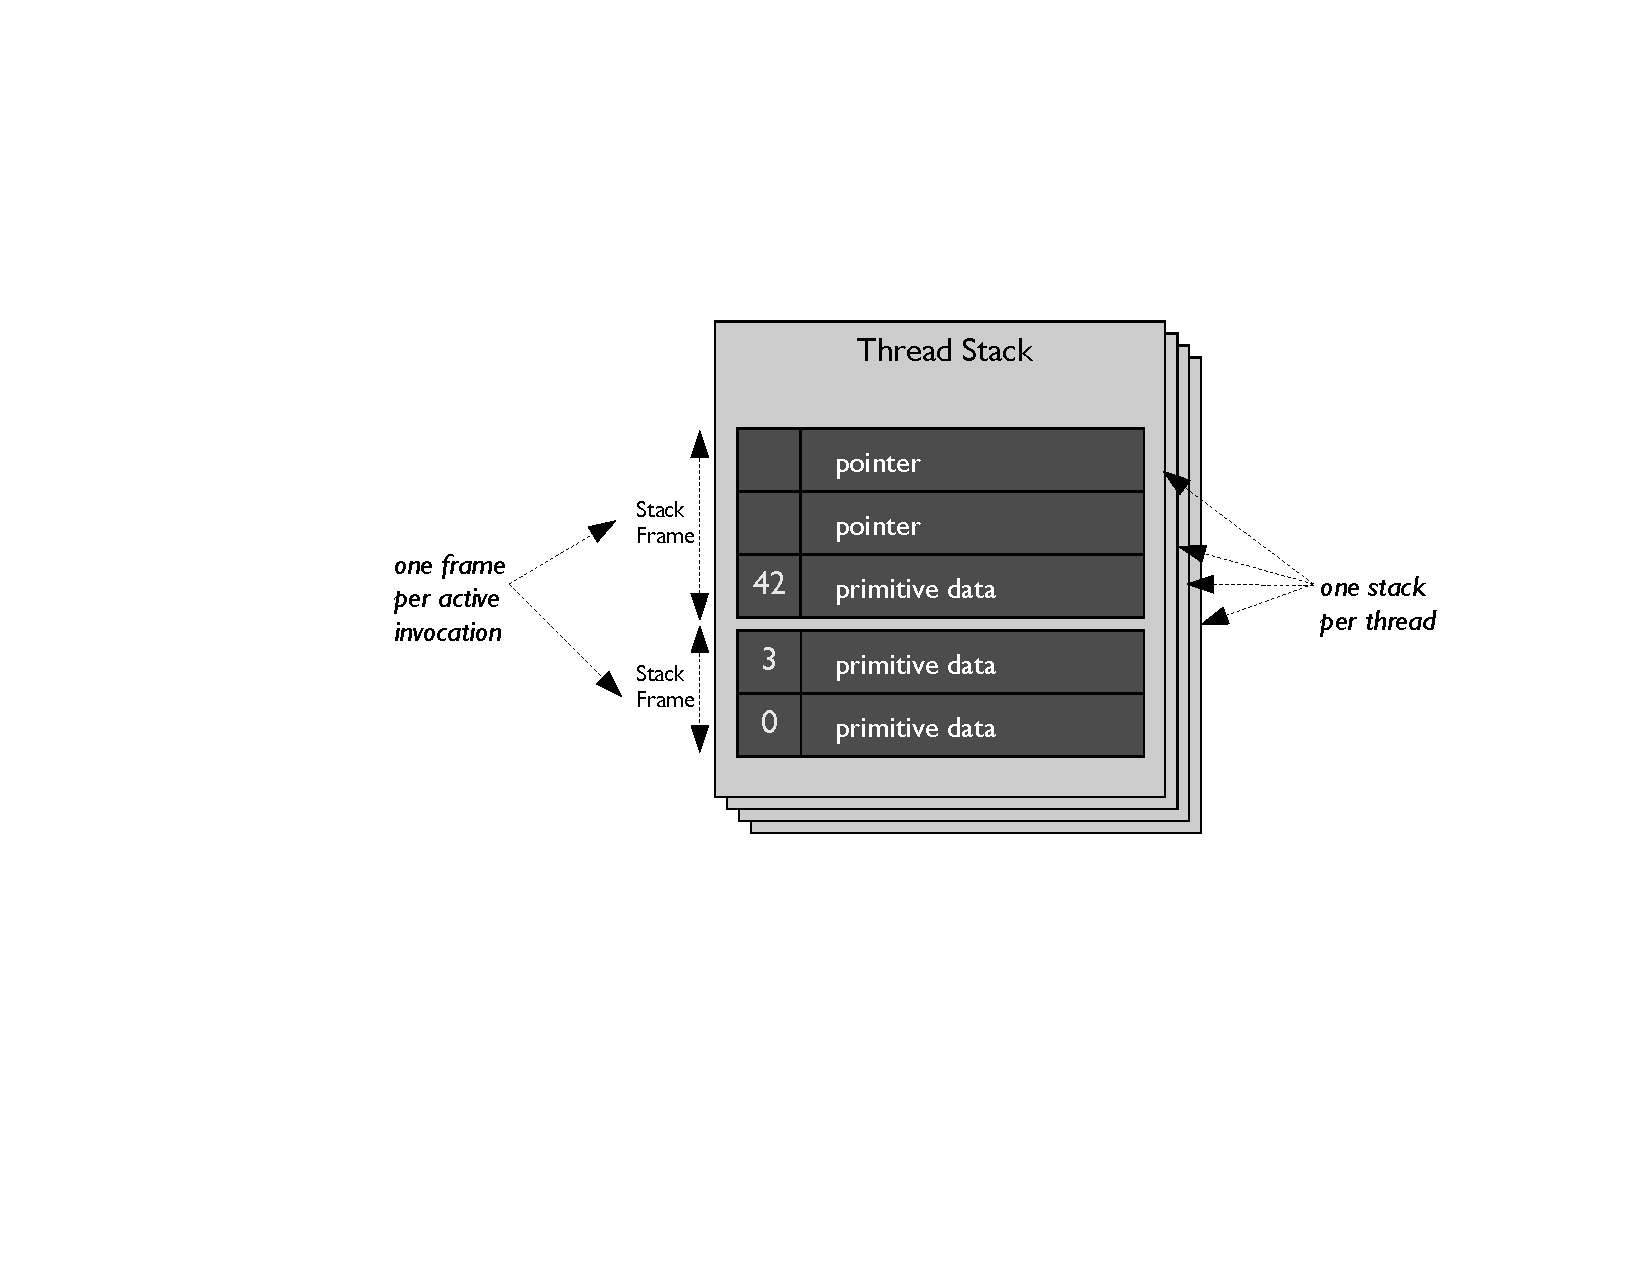
\includegraphics[width=0.7\textwidth]{part2/Figures/lifetime/heaps_and_stacks_stack_frames}
\caption{The compiler takes care managing the stack, by pushing and popping
the storage (called \emph{stack frames}) that hold your local variables and
method parameters.}
\label{fig:stack-frames}
\end{figure}

Like the heap, the stack also has limits to its size. Each thread in your
program can have a stack no deeper than a fixed limit, in bytes. If, during the
execution of a thread, these stack limits are exceeded, you may see a
\class{java.lang.StackOverflowError} exception
thrown\index{java.lang.StackOverflowError}. You can configure this property via
the {\tt -oss} command-line parameter.

%Most languages come with a minimal form of built-in memory management, in the
%form of the \emph{stack}.

%In Java, as shown in \autoref{fig:stack-frames}, each stack frame contains
%either primitive data or pointers to memory that has been allocated as a result
%of calls to {\tt new}. Unlike in a language such as C, you cannot dictate that
%the stack contain a structure, it can only contain pointers to structures that
%are stored on the heap. In C, when you write:
%\begin{shortlisting}
%struct {
   %int x;
%} g;
%
%g.x = 3;
%\end{shortlisting}
%the stack frame for this method will have one extra 32-bit slot, used to store
%the integer field {\tt x} of the local variable {\tt g}. 




% In Java, it is not possible for you to explicitly request that a structure be
\paragraph{A JIT Optimization: Stack Allocation}
Sometimes, the JIT compiler is clever enough to observe that a call to {\tt new}
can safely be allocated on the stack. This optimization is called \emph{stack
allocation} of objects\index{Stack Allocation}. It is enabled, by default, as of
Sun Java6 Update 21 and IBM 1.6 Service Release 2. When this optimization is
possible, objects created and used \emph{only} as local variables will be stored
on a stack frame; it is as if you were using C {\tt struct}s.
% \begin{shortlisting} class G {
   % int x;
% } G g = new G(); g.x = 3; \end{shortlisting} The JIT compiler attempts to
% determine whether that instance of {\tt G} will only be used in the method in
% which it was allocated, or whether it will ``escape'' and be accessible beyond
% the duration of the allocating invocation\index{Escape Analysis}. In many
% common cases, this is quite a difficult analysis task for the JIT. As soon as
% that {\tt g} is assigned to a field of some other object: \begin{shortlisting}
% H h = new H(); h.f = g; \end{shortlisting} then the compiler must now
% determine whether or not {\tt h} escapes. In most codes, objects are linked
% together in complex webs, which makes stack allocation applicable in only a
% limited set of cases. Unfortunately, there is no easy way to determine
% specifically which of your calls to {\tt new} will be, or were in any
% particular run, stack allocated by the JIT.
Though the JIT compiler can optimize away a fair number of short-lived objects
via stack allocation, you should not depend upon this optimization for your
long-lived data. It is a tricky thing for the JIT compiler to do correctly, and
so the compiler is very conservative in its application.\footnote{If you are
curious, the best you can do is to analyze performance both with and without the
underlying anlaysis. On Sun JVMs, you can disable the analysis by adding {\tt
-XX:-DoEscapeAnalysis} to your application's command line.}



%  a.b = new B();
%a.c = new C();
%a.b.d = new D();
%a.b.e = new E();
%a.b.e.f=new F();

\begin{comment}  
\begin{figure}
\begin{subfloat}
\begin{minipage}[b]{0.4\textwidth}
\begin{shortlisting}
class B {
  D d;
  E e;
}
void foo() {
  A a = new A();
  G g = new G();
  int x = 42;
  ...
}
\end{shortlisting}
\end{minipage}
\caption{A snippet of Java.}
\end{subfloat}
	\subfigure[Snapshot	of the heap and thread stacks.]
	{\label{fig:heaps_and_stacks_java}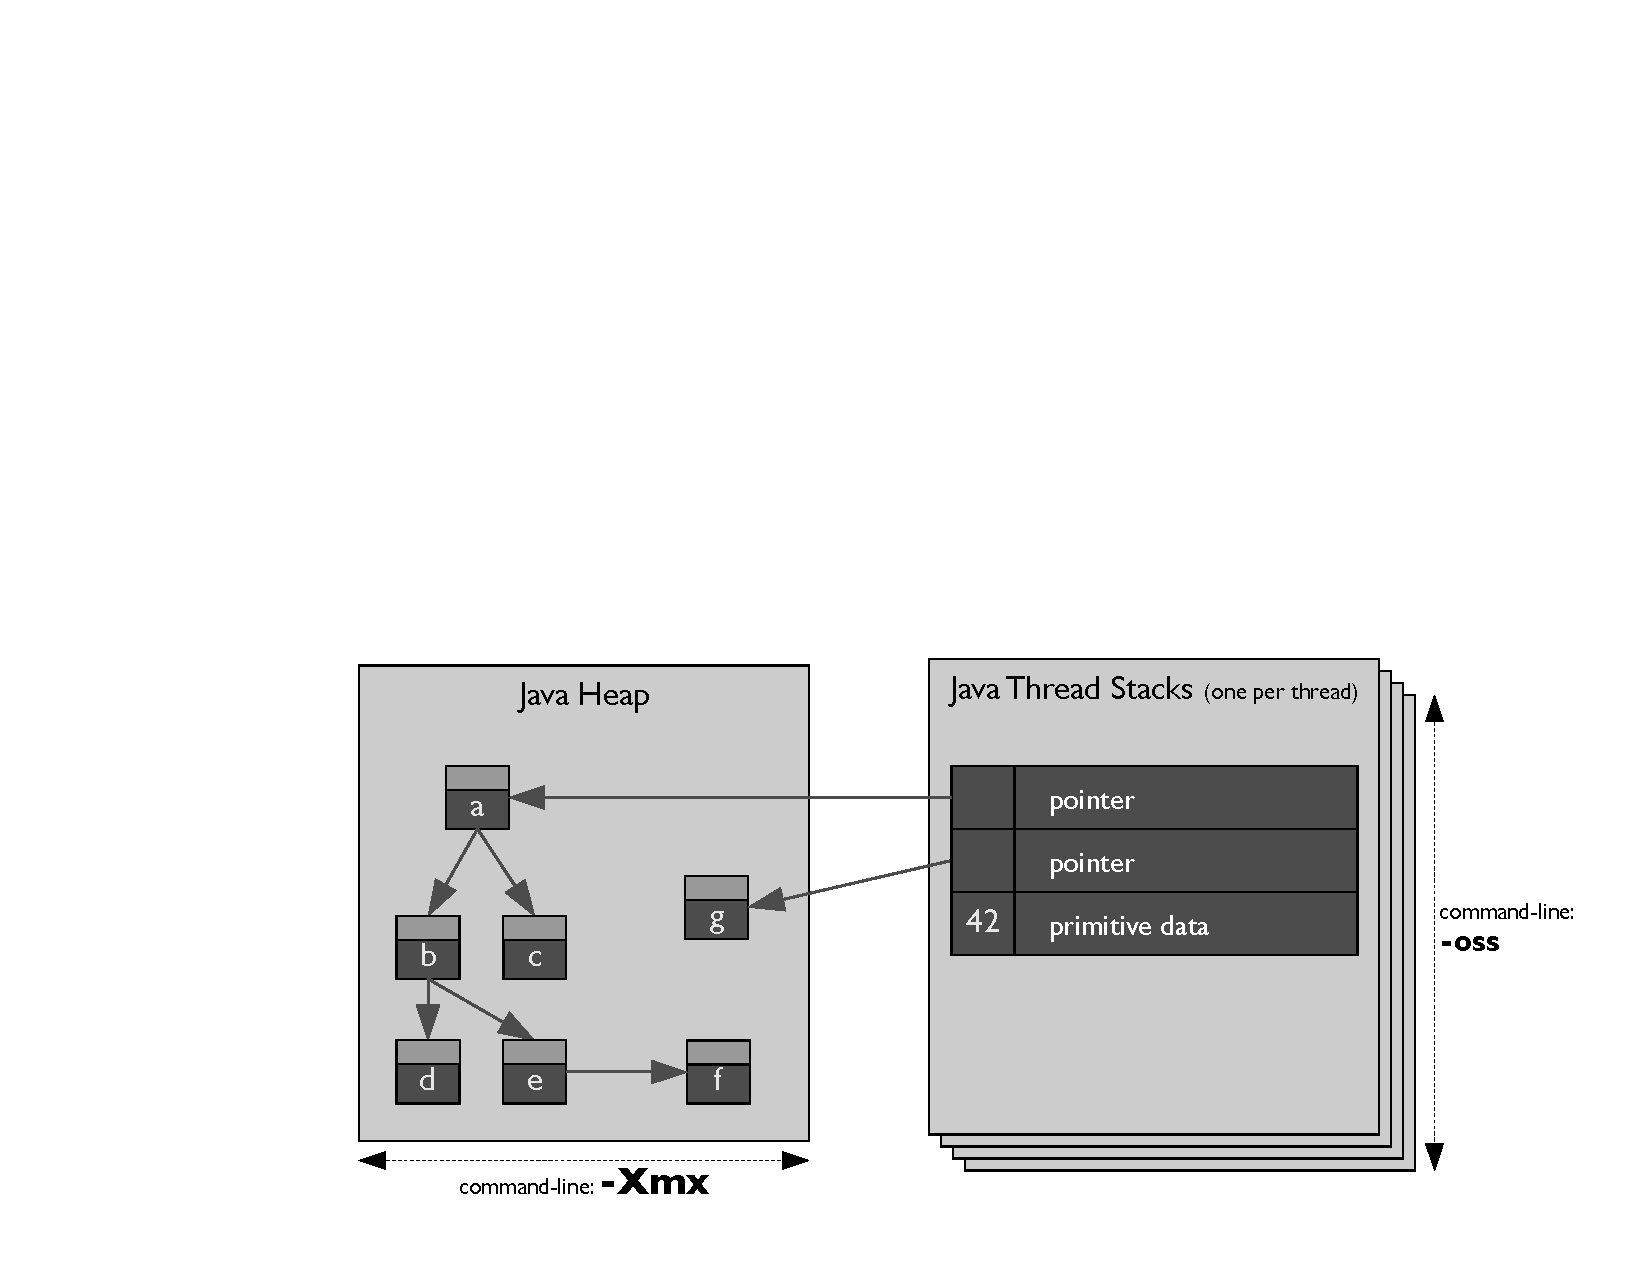
\includegraphics[width=0.575\textwidth]{part2/Figures/lifetime/heaps_and_stacks_java}} \caption{When using Java,
	the stack can
	contain only primitive data and pointers to heap objects; each of those heap
	objects has a header that the \jre tacks on, for its own management
	purposes.}
\end{figure}

\begin{figure}
\begin{subfloat}
\begin{minipage}[b]{0.4\textwidth}
\begin{shortlisting}
class B {
  D d; 
  E* e;
}
void foo() {
  A *a = new A();
  int x = 42;
  F f;
  G g;
  a->b->e->f = &f;
  ...
}
\end{shortlisting}
\end{minipage}
\caption{When coding in C++.}
\end{subfloat}
	\subfigure[When
	using
	native code, such as when coding in C,
	the stack can also contain allocated storage ({\tt
	structs}), and allocated storage can include
	other structures that have been inlined ({\tt d} has been inlined into {\tt
	b}); there are no headers in C, since it is not a managed language.
	]{\label{fig:heaps_and_stacks_C}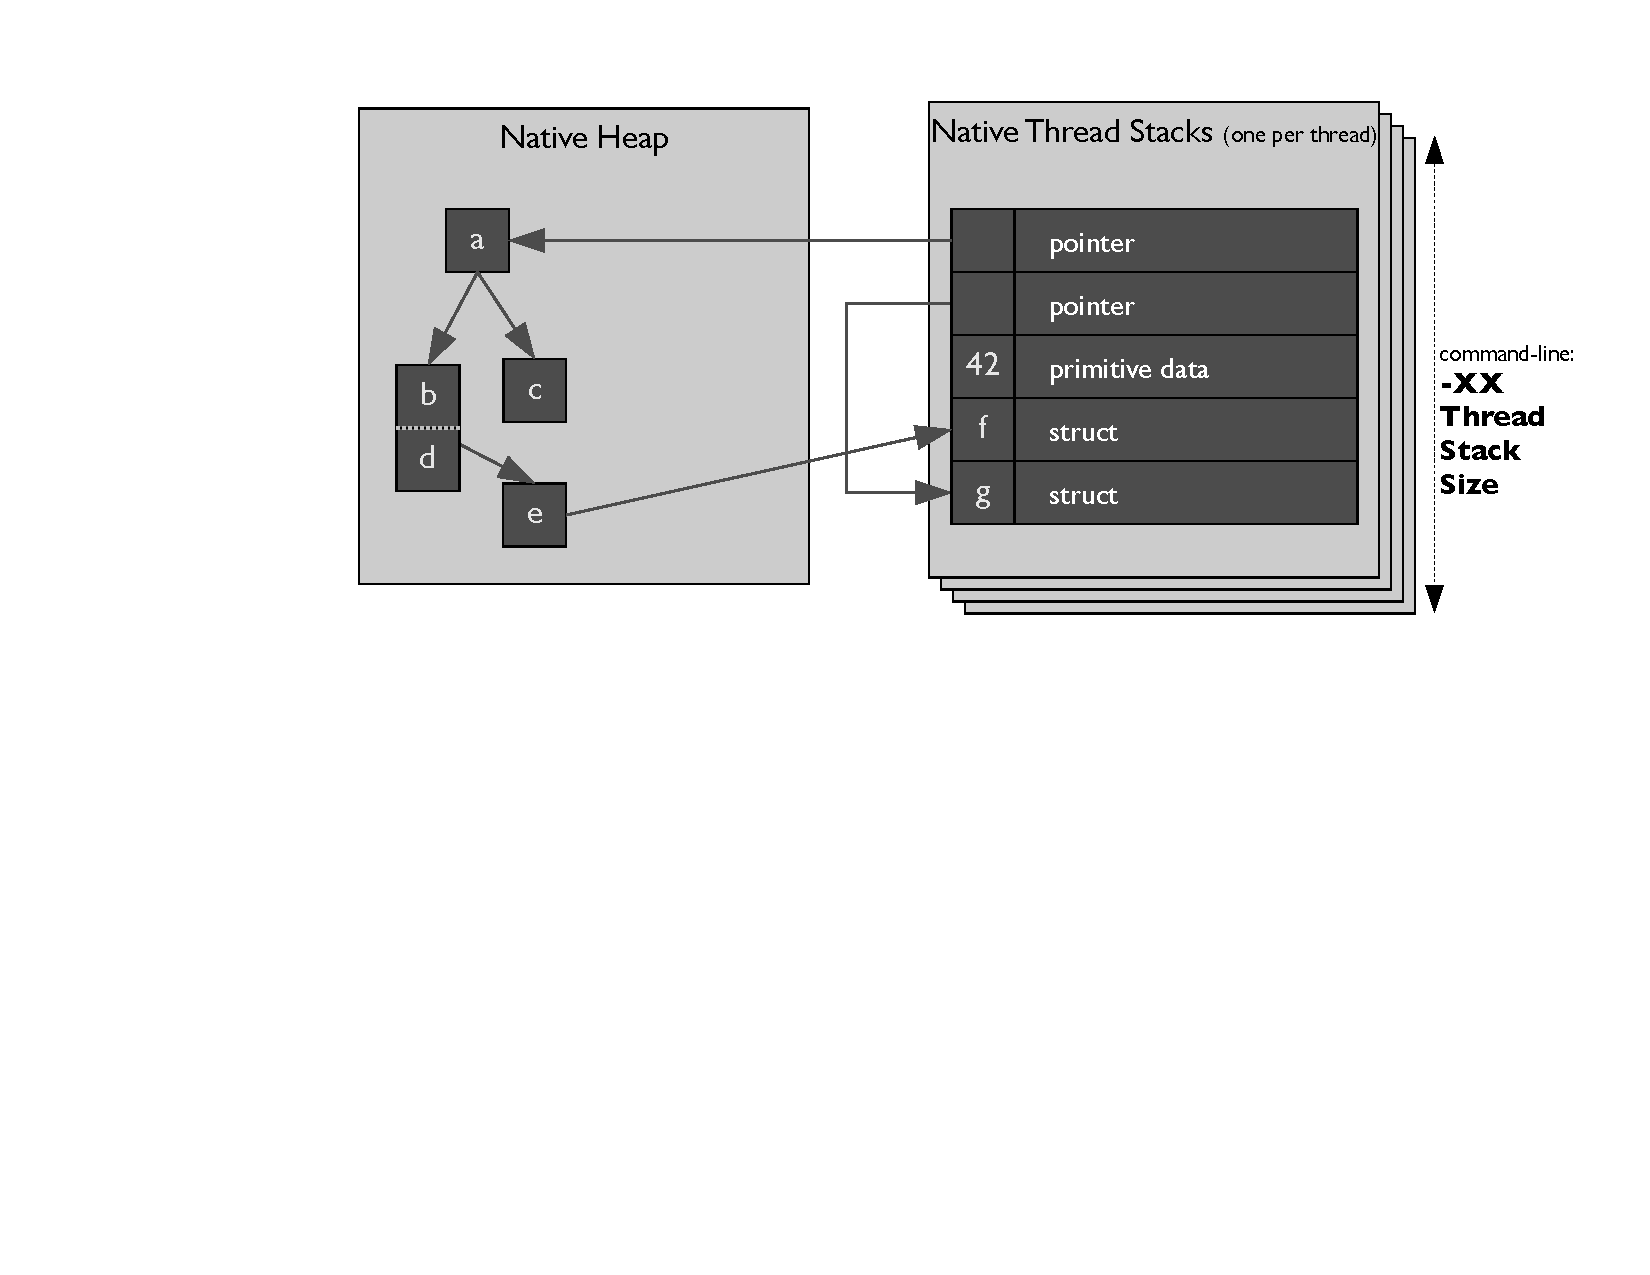
\includegraphics[width=0.575\textwidth]{part2/Figures/lifetime/heaps_and_stacks_C}}
\caption{Heaps and Stacks, in the C languge.}
\end{figure}
\end{comment}



\paragraph{Java Memory vs. Native Memory}
In addition to the heap and stack space that are devoted to Java data, every
Java program also has separate memory areas devoted to native data. The native
heap stores a variety of things, including memory allocations made by native
code that your application uses and the JIT compiled code of your application.
The \jre imposes an upper limit on the Java heap. In contrast, the operating
system sometimes imposes no limit on the size of the native heap. Therefore you
should be careful, and observe whether your application is indeed swapping any
native allocations to and from disk.

In addition, every thread in a Java program actually has two stacks, one for the
Java stack frames and one to hold the stack frames of any native methods that
either your Java code invokes or invokes your Java code. There is a command-line
parameter that you can use to configure the size of every native stack: {\tt
-ss}.

When your application exceeds any native limits you may confusingly see the same
error that you would see for exhaustion of Java memory resources: the {\tt
OutOf\-Memory\-Error}. Therefore, you should be aware of the Java and native
heap limits, in order to confirm the true source of the resource exhaustion: was it
due to running out of Java heap, or running out of native resources?


%The limits of the Java heap are determined by command-line parameters, as shown
%in \autoref{tab:stack-heap-limits}. The upper limit of native heap consumption
%is, for the most part, not directly controlled by parameters, but rather how
%much memory you have installed on your machine. The operating system will
%happily allocate to your application more and more memory, as it needs it.
%However, there are some important considerations that will sometimes constrain
%the consumption of native resources and, indirectly, the maximum size of the
%Java heap you can specify.

% is the table sufficient for this? or do we need exposition, too?
%To configure the
%maximum depth of the Java stacks to be 1 megabyte, you can add {\tt -oss1M} on
%your application's command line\index{Command-line arguments: -oss}\index{Java
%Stack, size limit}. To configure the maximum depth of the native stacks to be 1
%megabyte, you can add {\tt -ss=1M}\index{Command-line arguments: -ss}.


\paragraph{Physical Memory versus Address Space}
\index{Address Space}
Physical memory is one of the primary underlying constraints on how big you can
size your heaps. There is another limit that is independent of how much physical
memory you install on your machine. The limit depends on the number of memory
locations that can be addressesed, given the size of pointers on your machine.
The \emph{address space} of a process is the set of addresses that the process
can read or write via pointers. Therefore, this limit depends upon the size of
pointers on your platform, and, to a lesser extent, upon how the underlying
operating system. \autoref{tab:address-space-limits} gives some examples. If
your application runs on a 32-bit Windows operating system, the total amount of
memory that each process can access is 1.8 gigabytes\footnote{Some versions of
32-bit Windows let you specify a {\tt /3GB} boot option, which increases this
limit from 1.8GB to 3GB.} A pointer that is 32 bits wide can address 4
gigabytes, of which the operating system reserves roughly half for its own use.
If a process of your application attempts to allocate memory beyond this address
space limit, a failure will occur. It is quite often the case that this failure
will manifest itself misleadingly as a {\tt java.lang.OutOfMemoryError}.

\begin{table}
\centering
\begin{tabular}{rrc}
\toprule
%& \multicolumn{2}{c}{command-line parameter}\\
%memory area & min & max \\
Platform & Pointer Size & \shortstack{maximum memory\\consumption per process}
\\ \cmidrule(r){1-2} \cmidrule(l){3-3}
%Java stack &  & -oss \\
%Java heap & -Xms & -Xmx \\
%native stack & & -ss \\
z/OS & 31-bit & 1.3GB \\
Microsoft Windows & 32-bit & 1.8GB \\
UNIX-based & 32-bit & 2GB \\
Microsoft Windows & 32-bit {\tt /3GB} & 3GB \\
all & 64-bit & $\ge$ 256TB \\
\bottomrule
\end{tabular}
\caption{Even with plenty of physical memory installed, every process of your
application is still constrained 
  by the limits of the address space. On some versions of Microsoft Windows, you
  may specify a boot parameter {\tt /3GB} to increase this limit.}
\label{tab:address-space-limits}
\end{table}

Some operating systems let you specify limits on the amount of address space
that a process can use. This is similar to the way that you can specify {\tt
-Xmx} to limit the maximum amount of Java heap that a process should consume. On
UNIX platforms, you can use the {\tt ulimit} command. For example, on Linux, to
limit the amount of address space any process launched from the current shell
can access, say to 1 gigabyte, issue this command:
\begin{shortlisting}
% ulimit -m 1048576     // units in kilobytes
\end{shortlisting}
%You can also limit the size of the native stacks by issuing a similar command,
%except with the {\tt -s} flag.\index{ulimit} Very often, there are no memory
%limits by default. Native stack sizes are often limited to be in the megabyte
%range, per thread.

\paragraph{Native Resources: File Descriptors, etc.}
\index{Native Resources}
\index{File Descriptor Exhaustion}
Address space constraints exist on every operating system. Depending on your
operating system, there are often other resource limits that can lead to program
failures. For example, processes may be limited in the number of open files they
may have at any one time. You may see failures in your application, despite
having lots of memory and stack space free, because an application process has
exhausted file descriptors. On Windows platforms, there are other system-imposed
limits, such as the number of open font handles. You should be aware of these
common resource constraints, because they may impact the scalability of your
application. For example, you may have designed your application to keep many
font handles open for each thread, rather than keeping a common pool of them,
and sharing them across threads.

\section{The Garbage Collector}
The garbage collector is the mechanism for determining when an object should be
reclaimed. It is governed by a number of configuration choices that you can make.
These configuration choices guide the schedule that the collector follows. This
includes, for example, the frequency of collection and the lengths of pauses your
application experiences. In any case, the collector will obey some basic
principles, dictated by how your data structures are interconnected, when
determining \emph{what} to collect.

%\paragraph{What a Collection Collects: Reachability and Unique Ownership}
Each time a garbage collection occurs, the collector inspects the heap for
possibly \emph{live} objects. The collector treats the heap as a graph of
objects. The nodes are the objects themselves, and the edges are field or array
slots that result in a pointer from one object to another. \index{Heap, as a
graph of objects} Recursively, an object is live either if it is a referenced
either by a live object, or, in the base case, by a \emph{root}. The roots of
garbage collection are those that come from outside the Java space, and include:
objects serving as monitors, objects on the stack of a method invocation in
progress, and references from native code via the Java Native Interface (JNI).
Every other object not live, in this sense, are ready for collection; they are
garbage.

\begin{figure}
\centering
	\subfigure[A live data
	structure.]{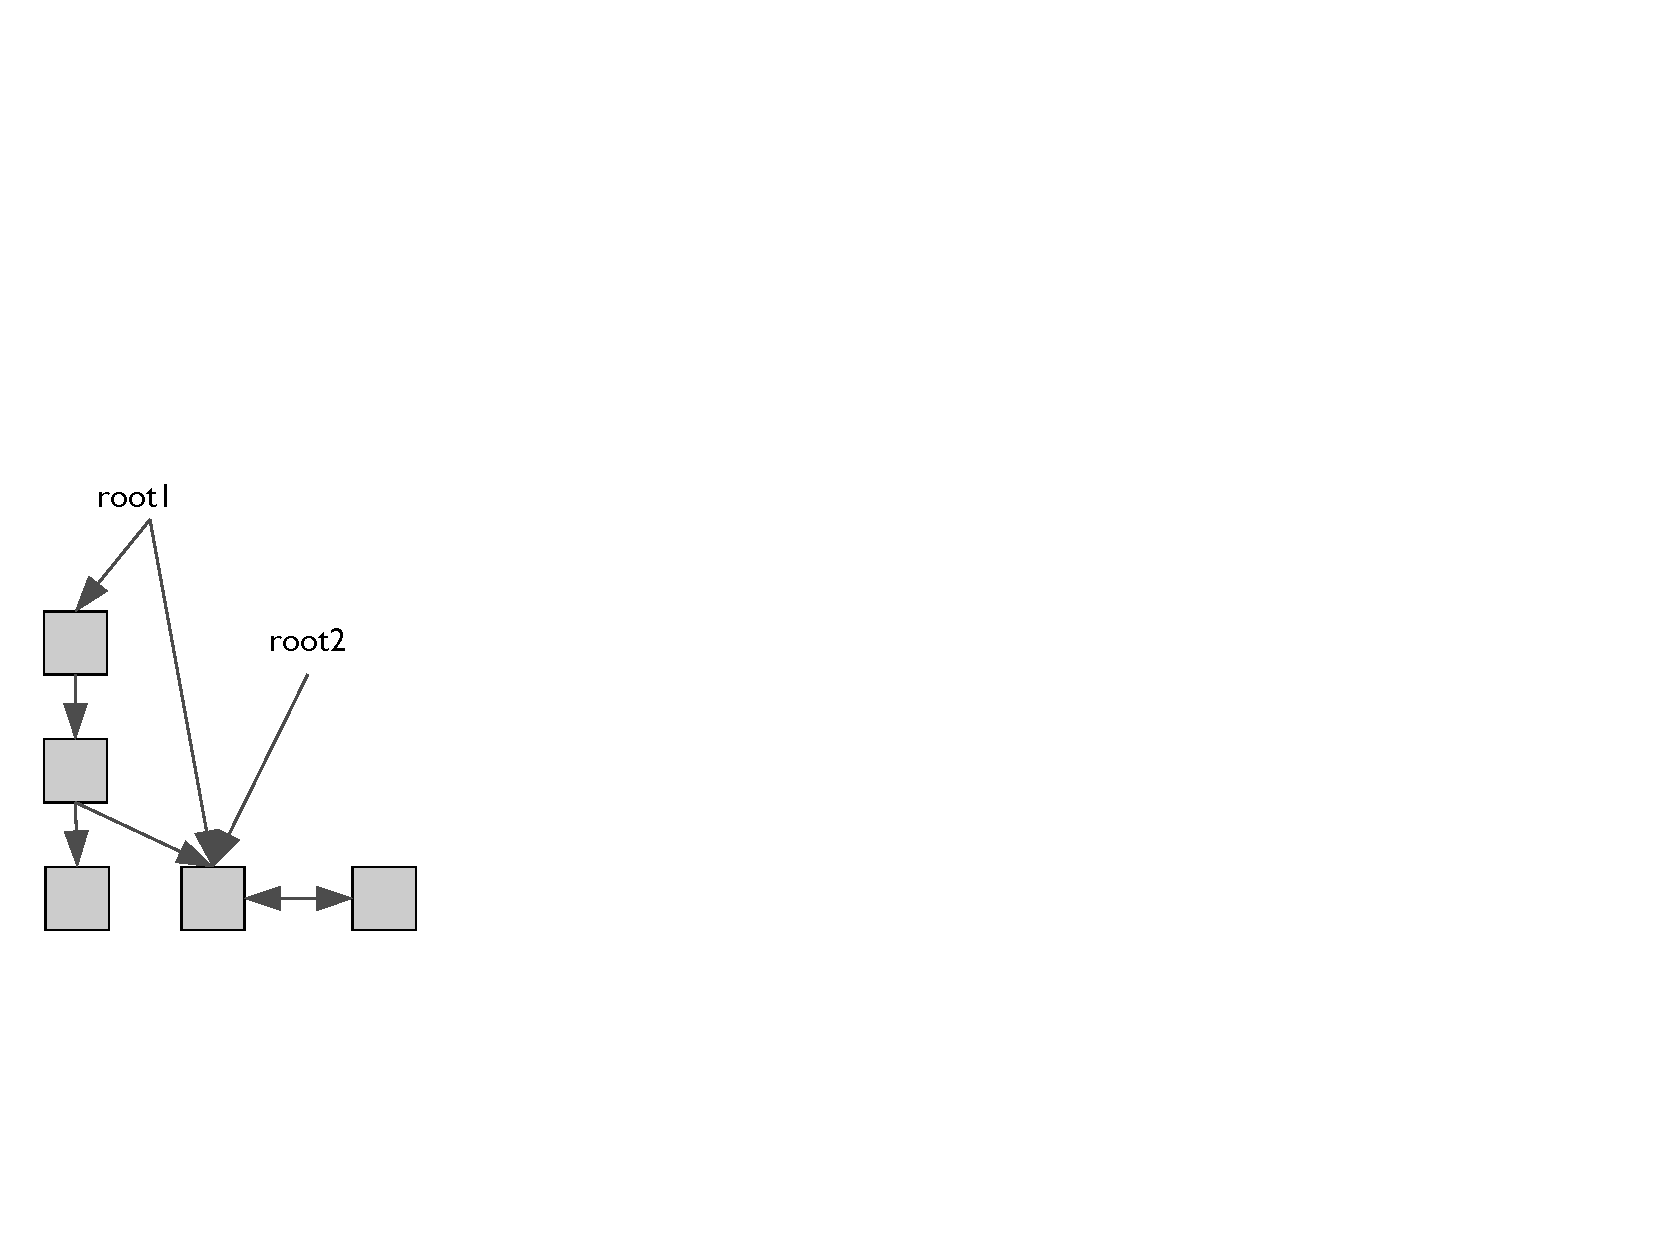
\includegraphics[width=0.3\textwidth]{part2/Figures/lifetime/reachability1}}
	\hspace{0.18\textwidth}
	\subfigure[Then, the dominating reference is
	clipped.]{\label{fig:reachability-b}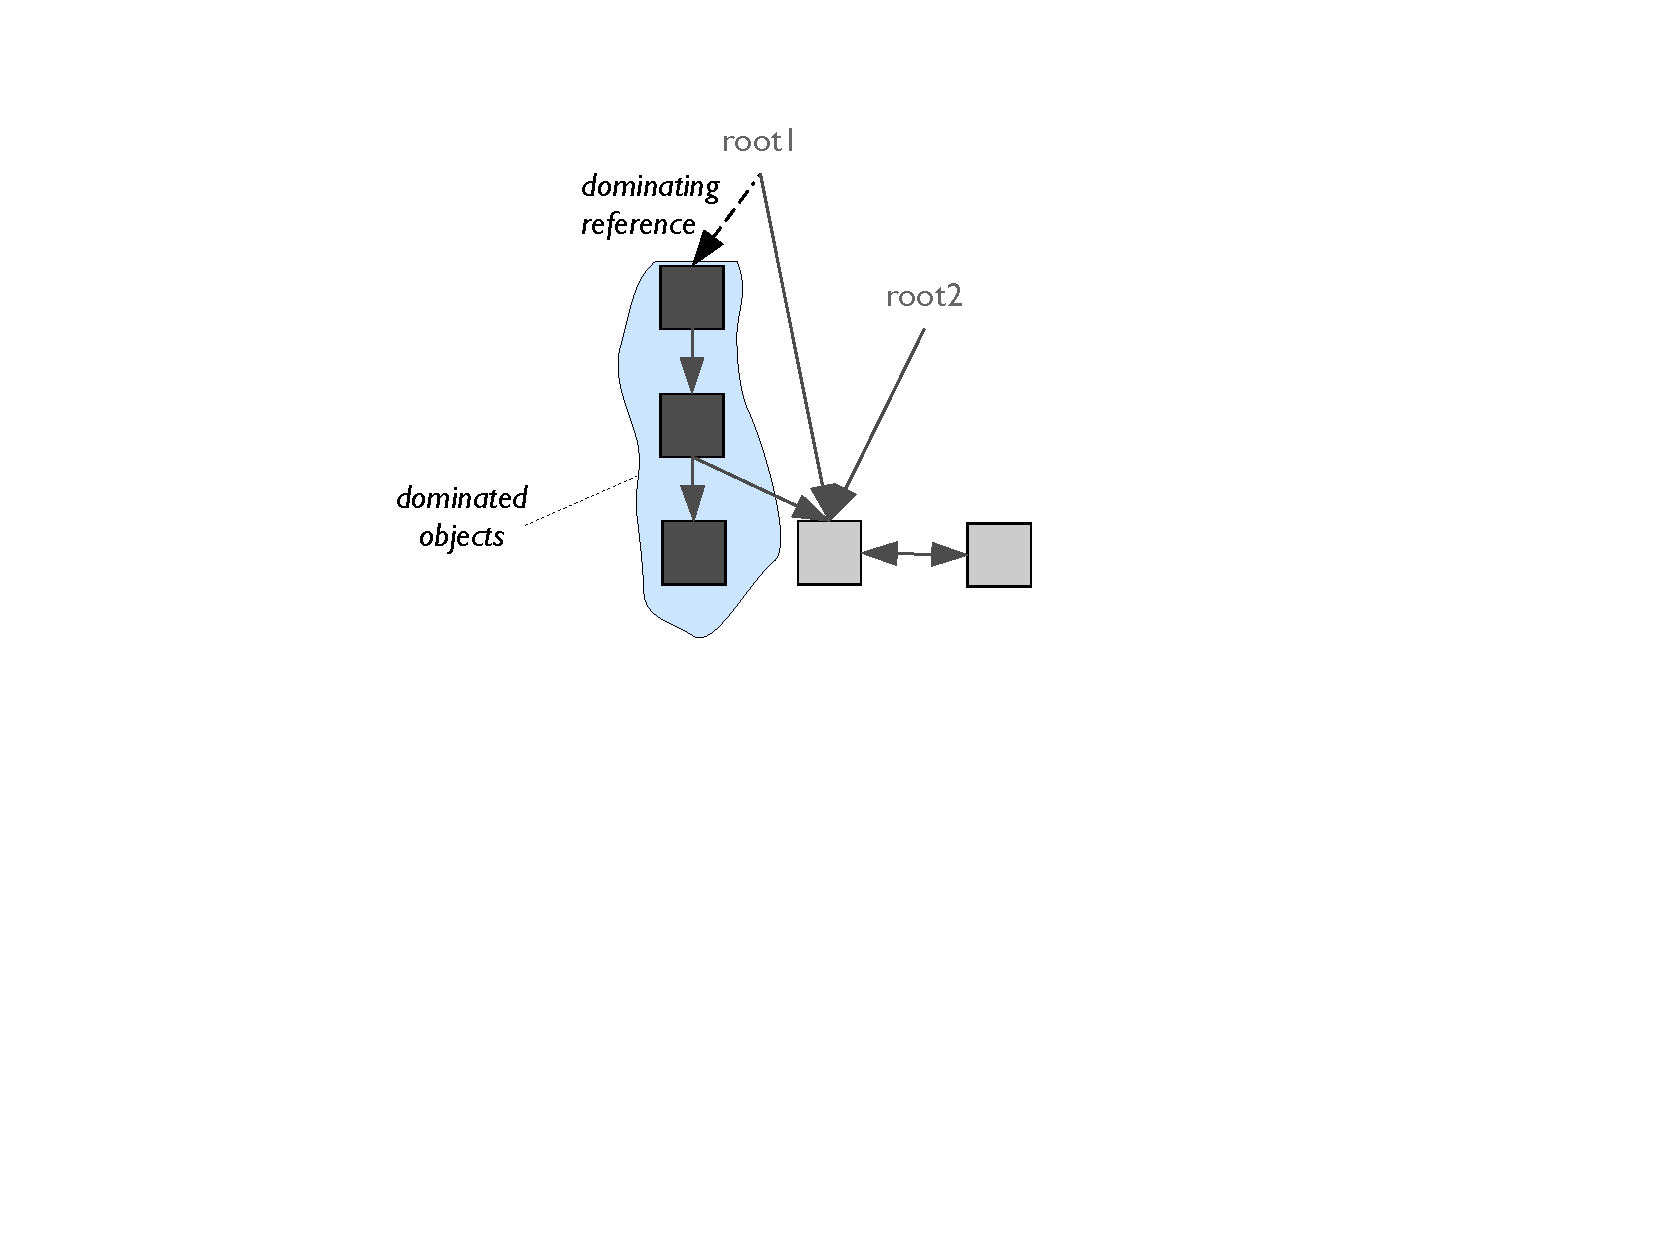
\includegraphics[width=0.445\textwidth]{part2/Figures/lifetime/reachability2}}
	\caption{The garbage collector uses the references between objects to
	determine what objects are collectable. The data structure on the left is
	filled entirely with live objects. The one on the right, after a link is
	clipped, now contains some collectable objects; all objects reachable only by
	traversing a \emph{dominating reference}, i.e. those \emph{dominated objects},
	will be collectable, as well.}
	\label{fig:reachability}
\end{figure}

This recursive aspect can also be expressed in terms of \emph{reachability}.
\index{Reachability} The live objects are those objects reachable, by following a
chain of references, from some root. \autoref{fig:reachability} illustrates a
simple data structure, and shows which part becomes collectable when a reference
is set to null, or ``clipped''. When the indicated reference is clipped, there is
no chain of references from a root to the shaded region of objects.

Reachability is the graph property that determines what objects are still live.
This is all the garbage collector cares about, finding the objects that need to
be kept around. It is also helpful for programmers to know which objects become
dead as the result of a pointer being clipped. The objects within the shaded
region of \autoref{fig:reachability-b} have the property that each is reachable
\emph{only} from the clipped reference. That clipped reference is the unique
owner of the shaded objects. The graph property that describes unique ownership
is called \emph{dominance}; \index{Dominance} the clipped reference is said to
dominate those objects that it uniquely owns.

\section{The Object Lifecycle}
\paragraph{How to Free an Object in Java}
\label{sec:natural-lifetime}
\index{Natural Lifetime of Objects}

If you wish an object's storage to be reclaimed, you must take some care. To do
so in a language like C is simple, if bug prone. When you call \code{free} on any
pointer to a dynamically allocated memory region, memory is immediately available
for subsequent use.\footnote{It is possible to run a C program with a
special \code{malloc} library that introduces a simplified form of garbage
collection.} A C style of memory management comes with well known risks, and
commonly leads to memory errors. For example, memory might be deallocated more
than once, or variables that do not point to the start of an allocated region
might be passed to \code{free}. Still, using \code{free} is straightforward to
use, and immediate in effect.

In Java, you are immune from these problems, but there is no way to return memory
for immediately use in future allocations. Instead, you indicate, either
implicitly or explicitly, that objects are no longer needed. The explicit
mechanism is to set references to null. To do so implicitly, there are several
devices at your disposal. This section describes the details of both.

It is important to remember that in contrast to C, all means of indicating an
object is no longer needed have a certain degree of delay. There are delays of
two sorts. First, if you rely on the implicit mechanisms for indicating an object is no
longer needing, there is often a delay from its last use to this point. Second,
there is a delay from the point at which you indicate an object is no longer
needed until its storage is reclaimed.

\paragraph{The Lifecycle of an Object}
These two delays are but a part of the larger lifecycle that every Java object
goes through, from creation to reclamation. In a well-behaved application, an
object's lifetime spans its allocation, use, and the short period during which
the \jre takes control and reclaims the space. For some subset of an object's
actual lifetime, that is the time from creation to reclamation, your application
will make use of the data stored in its fields. \autoref{fig:typical-lifecycle}
illustrates the lifecycle of a typical object in a well behaved application.

\begin{figure}
	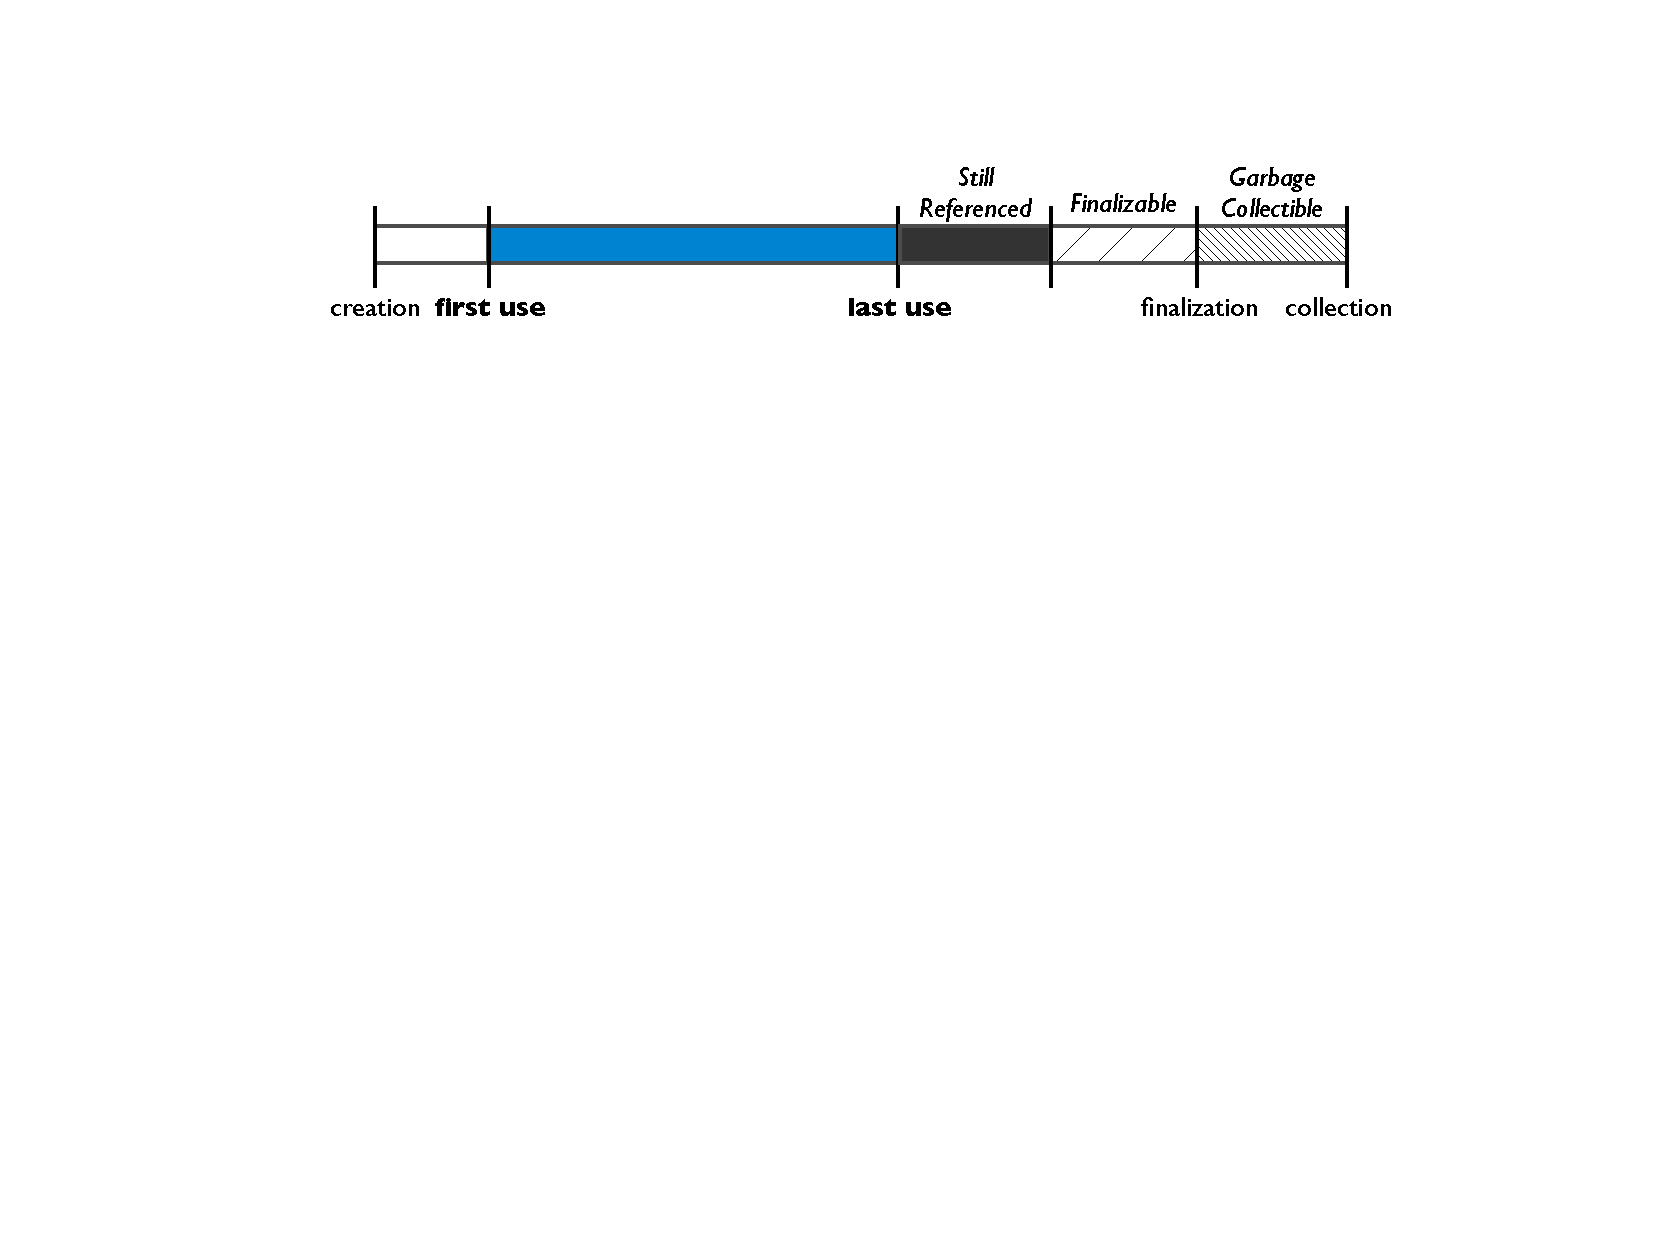
\includegraphics[width=0.9\textwidth]{part2/Figures/lifetime/object-lifecycle}
	\caption{Timeline of the life of a typical object.}
	\label{fig:typical-lifecycle}
\end{figure}


\begin{example}{Parsing a Date} Consider a loop that shows an easy way to parse
a list of dates. What objects are created, and what are their lifetimes?
\begin{shortlisting}
for (String string : inputList) {
	ParsePosition pos = new ParsePosition(0);
	SimpleDateFormat parser = new SimpleDateFormat();
	System.out.println(parser.parse(string, pos));
}
\end{shortlisting}
\end{example}

For each iteration of this loop, this code takes a date that is represented as a
string and produces a standard Java \class{Date} object. In doing so, a number of
objects are created. Two of these are easy to see, in the two \code{new} calls
that create the parse position and date parser objects. The programmer who wrote
this created two objects, but many more are created by the standard libraries to
finish the task. These include a calendar object, number of arrays, and the
\class{Date} itself. None of these objects are used beyond the iteration of the
loop in which they were created. Within one iteration, they are created, almost
immediately used, and then enter a state of drag.

\callout{drag}{Memory Drag}{
\index{Drag}
At some point, an object will never be used again, but the \jre doesn't yet know
that this is the case. The object hangs around, taking up space in the Java heap
until the point when some action is taken, either by the \jre or by the
application itself, to make the object a candidate for reclamation. The interval
of time between its last use and ultimate reclamation is refered to as
\emph{drag}.}

The \code{pos} object represents to the parser the position within the input
string to begin parsing. The implementation of the \code{parse} method uses it
early on in the process of parsing. Despite being unused for the remainder of the
parsing, the \jre does not know this until the current iteration of the loop has
finished. For this duration of time the object is in a kind of limbo, where it is
referenced but never be used again. This limbo time also includes the entirety of
the call to \code{System.out.println}, an operation entirely unrelated to the
creation or use of the parse position object. Once the current loop iteration
finishes, these two objects will become candidates for garbage collection.
The object now enters a second stage of this limbo. There are no pointers to
{\tt pos} that should keep its memory around, but the memory will stay around
until the next garbage collection.
Only when the garbage collector performs a sweep over memory, looking
for reclaimable objects, will the memory for {\tt pos} be ready for new objects.
Most of the time, this second stage of limbo is short, because garbage
collections typically run ever few seconds.

However, if there is a long interval
of time during which your application allocates very few objects in the Java
heap, it could be quite a while before these dragging objects are reclaimed. You
should be cautious here if, during these lulls in Java object creation, your
application is heavily exercising the native heap. If your application has a few
Java objects that implicitly reference native resources that are constrained,
you could run into trouble. For example:
\begin{shortlisting}
Font f = 
\end{shortlisting}

\begin{figure}
	\centering
	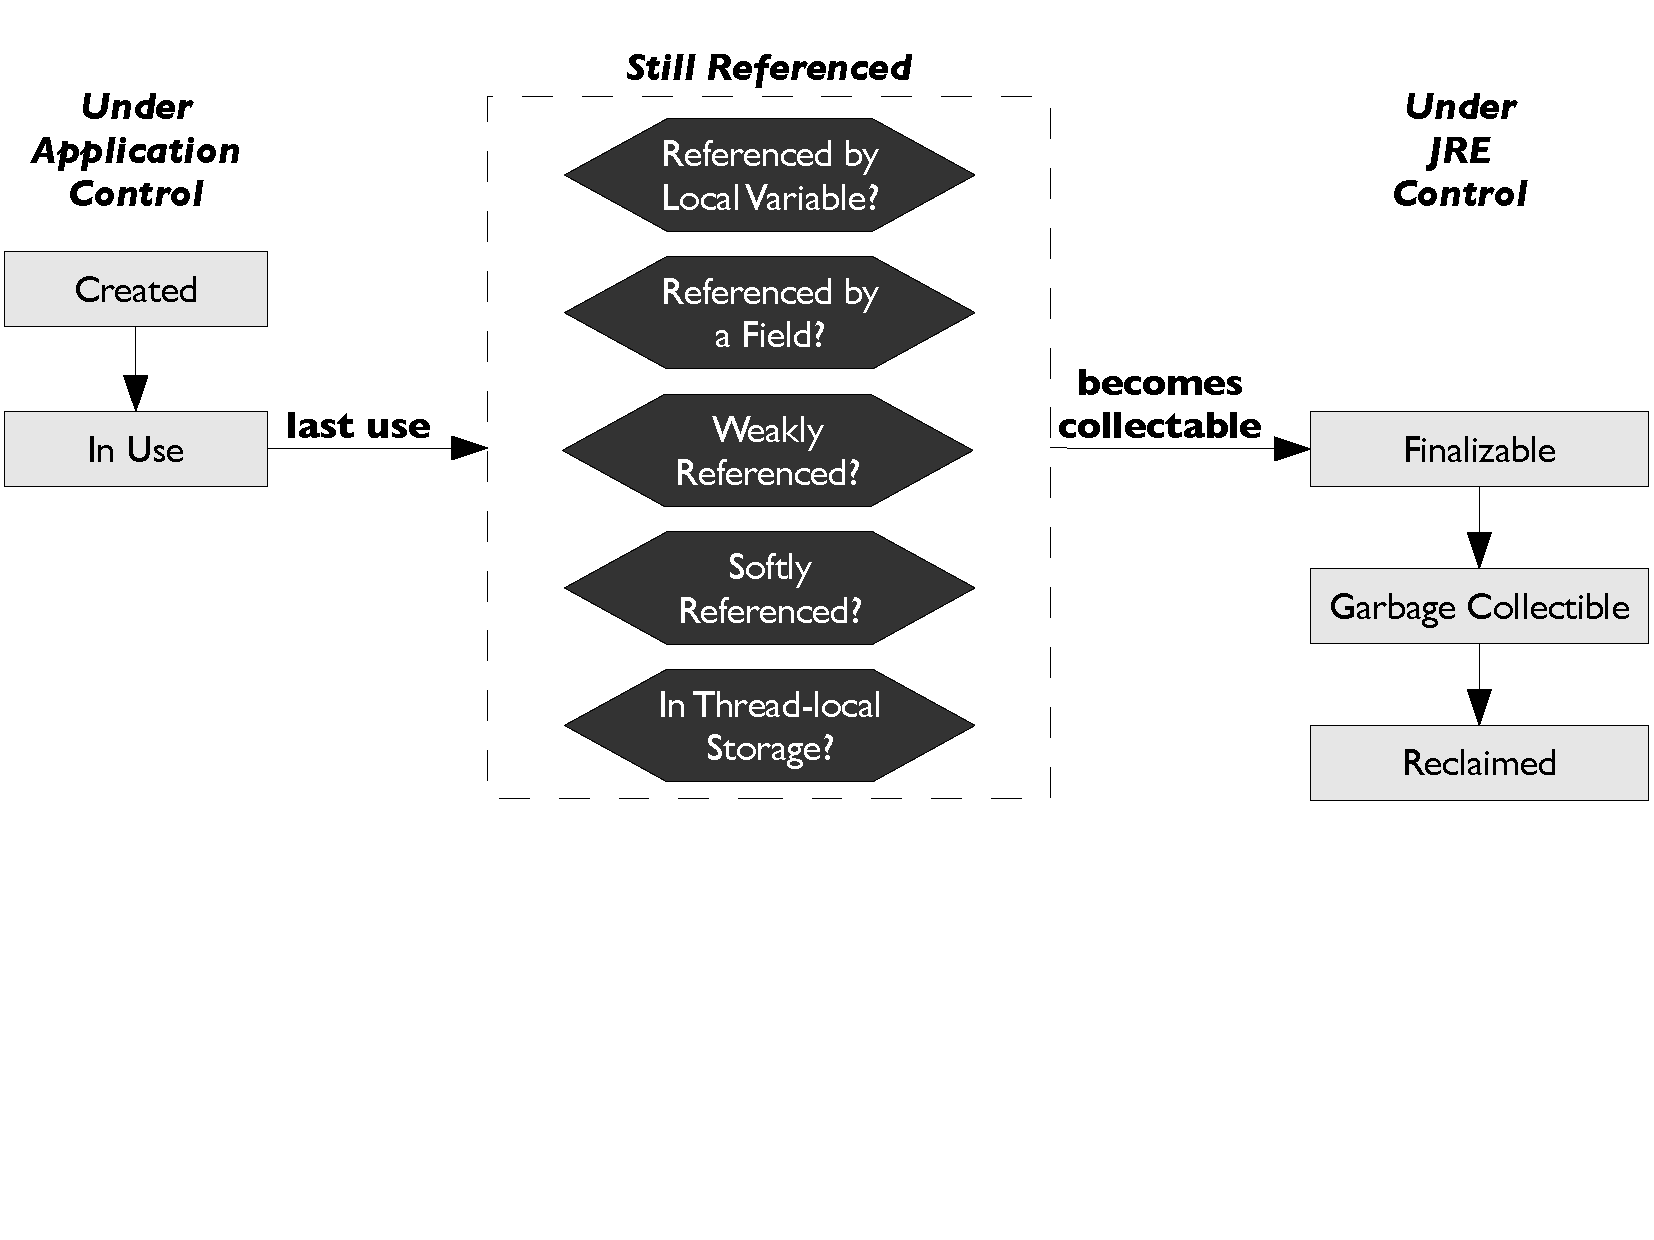
\includegraphics[width=\textwidth]{part2/Figures/lifetime/states}
	\caption{After its last use, an object enters a kind of limbo: the application
	is done with it, but it is not yet a candidate for garbage collection. When an
	object exits this limbo depends on the way it is referenced by your
	application.}
		\label{fig:limbo-exit}
\end{figure}

Depending on how the object is referenced by your application, it will
transition from in-use to garbage-collectable in a different manner. There are
eight ways an object may be referenced. It can be referenced by a:

\begin{enumerate}
  \item local variable of a method
  \item static field of a class
  \item instance field of a \class{java.util.ref.WeakReference} object
  \item instance field of a \class{java.util.ref.SoftReference} object
  \item instance field of a \class{java.util.ref.PhantomReference} object
  \item \tls
  \item instance field of any other object
  \item some combination of the above
\end{enumerate}

The first seven are cases of unique ownership of an object. There exists
only one path, via that particular reference, to reach the object. The eight case
is one of \emph{shared} ownership. After your program creates an object, it
references the object in one or more of these eight ways. The ownership of an
object may vary over time --- as your program runs, these references will come
and go. After some time, program execution may reach a point where the object is
no longer under application control. At this point, the \jre is now in charge of
its lifetime. For example, if the only reference to an object is from a field of
some other object, and your code reassigns that reference to \code{null}, this
becomes a point of transition, from application control to \jre control. Each of
the eight ways of referencing an object comes with its own guidelines as to when
this transition occurs. \autoref{fig:limbo-exit} %and \autoref{tab:limbo-exit}
summarizes how an object transitions to \jre control. The following code gives
examples of these eight patterns of ownership:
\lstset{numbers=left,numbersep=12pt,numberstyle=\tiny\textsf}
\begin{shortlisting}
class Foo {
   void bar(Object argument) {
      Object localVariableReference1 = new ...;
      threadLocal1.set(argument);
      threadLocal2.set(new ...);
      localVariableReference1 = null;
      for (...) {
         Object localVariableReference2 = new ...;
         ...
      }
   }

   static Object staticField = new ...;
   Object instanceField = new ...;
   Reference weak = new WeakReference(instanceField);
   Reference soft = new SoftReference(instanceField);
   Reference phantom = new PhantomReference(instanceField);
   ThreadLocal threadLocal1 = new ThreadLocal();
   ThreadLocal threadLocal2 = new ThreadLocal();
}
\end{shortlisting}
\lstset{numbers=none}
% Still, one can't always rely on automatic mechanisms to guide an object out of
% limbo in a timely fashion.

\begin{comment}
\begin{table}
\centering
	\begin{tabular}{ll} \toprule uniquely owned by  & 
	when object becomes candidate for reclamation \\ \cmidrule(r){1-1}
	\cmidrule(l){2-2}
			%
			nothing & immediately
        	\\
        	%
        	local variable & after scope exits, e.g. method returns
        	\\ \addlinespace
        	%
        	instance field of an object & 
        	when that object becomes reclamation candidate
        	\\
        	%
        	static field of a class &
        	when that class is unloaded
        	%
        	\\ \addlinespace
        	field of \class{WeakReference} & immediately
        	%
        	\\
	       	\ldots with \class{ReferenceQueue} &
        	immediately placed on queue, then after queue is polled
        	%
        	\\ \addlinespace
        	field of \class{SoftReference} & approximately
        	LRU%$^{**}$
        	%
        	\\
	       	\ldots with \class{ReferenceQueue} &
        	after LRU, placed on queue, then after queue is polled
        	%
        	\\ \addlinespace
        	entry in \tls & when that thread dies
        	%
        	\\ 
        \bottomrule
    \end{tabular}
	\caption{When an object becomes a candidate for reclamation. The dominating 
	reference can be explicitly overwritten, e.g. by your code expliclty assigning the
	reference to \code{null}. Otherwise, an object only automatically becomes a
	candidate under the restricted circumstances shown here.
%	The point when an object exits limbo depends on 
	%decisions under programmer control: it depends on how the object is
	%referenced.
	%older {\jre}s	use very poor heuristics for handling soft references; see the
	% body for more detail.
	%, it will be reclaimed
	%under certain rules, or may be part of a memory leak
	}
	\label{tab:limbo-exit}
\end{table}
\end{comment}

\paragraph{The Lifetime of Local Variables}
\label{sec:lifetime-of-locals}
Variables that are declared within a method body often have a lifetime that is
bound to, at most, the duration of an invocation of that method.
% If an object is uniquely owned by a local variable of a method, the \jre will
% begin to consider reclaming its storage no sooner than when the local
% variable's scope exits.
Common examples of this are local variables, loop variables, and variables
declared within some inner scope such as within the body of a loop or \code{if}
statement. For these variables, when a loop continues to the next iteration as in
the case of \code{localVariableReference2}, when the body of a clause of an
if/then/else statement finishes, or when the method invocation returns as in the
case of \code{localVariableReference1}, there is a good chance that the object
referenced by that variable will be reclaimable.

There are situations where an object may \emph{escape} the local scope in which
it was declared.\index{Escaping Objects} In these cases, the object has
\emph{shared ownership}\index{Shared Ownership} until this local scope exits.
See below for further discussion of shared ownership. This is an example of an
object escaping a local variable scope, so that it is, for the duration of that
local scope, also owned by a static field of a class object:
\begin{shortlisting}
class Foo {
   static Object static_obj;
   
   void foo() {
      Object obj = new Object();
      static_obj = obj;
      ... // uses of obj
   } // obj scope exits, but static_obj ownership persists
}
\end{shortlisting}
The next section discusses the lifetime of static fields.

The minimum that the Java language specification requires is that non-escaping
objects that are declared within some scope inside of a method will be
reclaimable by the time that scope exits. Many modern \jres try to optimize by
inferring, when they can, the line of code at which an object will certainly
never be used again. For this reason, some (but not all!) sources of memory
drag\index{Drag} that would have been a problem with older \jres, are no longer
an issue. For example, you can run this test program and, by inspecting the
output, determine whether your \jre is performing this kind of optimization:
\begin{shortlisting}
/* Test for whether the optimizer detects that obj is reclaimable before the end of this method */
static public void main(String[] args) {
   Object obj = new Object() {
      protected void finalize() {
         System.out.println("Finalized");
      }
   };
   System.out.println("StartOfLoop");
   for (int i = 0; i < 1000000; i++) {
       new HashSet().add(i);
   }
   System.out.println("EndOfLoop");
}
\end{shortlisting}
If you see the \code{Finalized} message before the end of loop message, this is a
sure sign that the \jre is being clever. Be careful to remember that seeing the
finalized message is definitive evidence, but not seeing that message might only
mean that your loop doesn't iterate enough times to cause a garbage collection to
occur. You may need to experiment with the number of loop iterations, before
coming to a conclusion.

\paragraph{The Lifetime of Statics, and Class Unloading}
\index{Class Unloading}
\index{Static fields}

The \jre allocates memory for every class, to store its static fields, such as
the one on line 13 in the above example. This memory, to store all static fields
plus some bookkeeping information, is often referred to as the \emph{class
object} for the class.\index{Class Objects} It is possible for the same class to
be loaded into multiple class loaders; in this way, using more than one class
loader lets you avoid the problem of colliding use of static fields in separately
developed parts of the code. A static field therefore only exits scope when the
class object is reclaimed, which occurs when the respective class is unloaded, by
the \jre, from its class loader. 

If a class is never unloaded, which is likely to the be case for your
application, then that class object will remain permanently resident. The
\emph{default} class loader, which is the one that will be used unless you
specify otherwise, never unloads application classes. 

If you need classes to be unloaded, then you must manually specify a class loader
to use. Unloading a class is then accomplished by ensuring that all references to
both the class object and your custom class loader, are set to \code{null}. This
will render the class unloadable, and will also render objects referenced by
static fields all classes loaded into that class loader as garbage collectable.
There exist module management systems, such as OSGi~\cite{OSGi_2007}, that
facilitate this task.

Due to these complexities, your design should generally anticipate that the
memory for these static fields is permanently resident. This means that any
static fields referencing an instance, rather than containing primitive data,
will render that instance also permanently resident. Unless, that is, you take
action to explicitly clip the static field reference, by assigning the field to
null. Otherwise, that instance will be forever reachable along a path from some
garbage collection root through the static field reference. In this way, storing
a reference in a \code{static} field of an class is one way to implement a
permanently resident lifetime policy.

\paragraph{The Lifetime of Instance Field References}

As long as an object \code{B} is dominated by an instance field of another
object \code{A}, then \code{B} will live as long as \code{A} does, and become
collectible whenever \code{A} does. The only device at your disposal to make
\code{B} garbage collectable before \code{A} is to break all paths of references
from \code{A} to \code{B}. In simple cases, where \code{B} is directly
referenced by a field of \code{A}, then reassigning that reference to
\code{null} will do the trick. After doing so, the \code{B} object will now be a
candiate for garbage collection.



%Every object created by your application lives for an interval of time from its
%creation to the point that the Java runtime gets around to collecting it. An object's {\em natural} lifetime is defined by the
%interval of time between its first and last necessary use. %cite drag paper
%here?








\begin{comment}
\begin{figure}
	\centering
%	\subfigure[The lifecycle of a typical object and its data.]{
	%\label{fig:typical-lifecycle1}
			%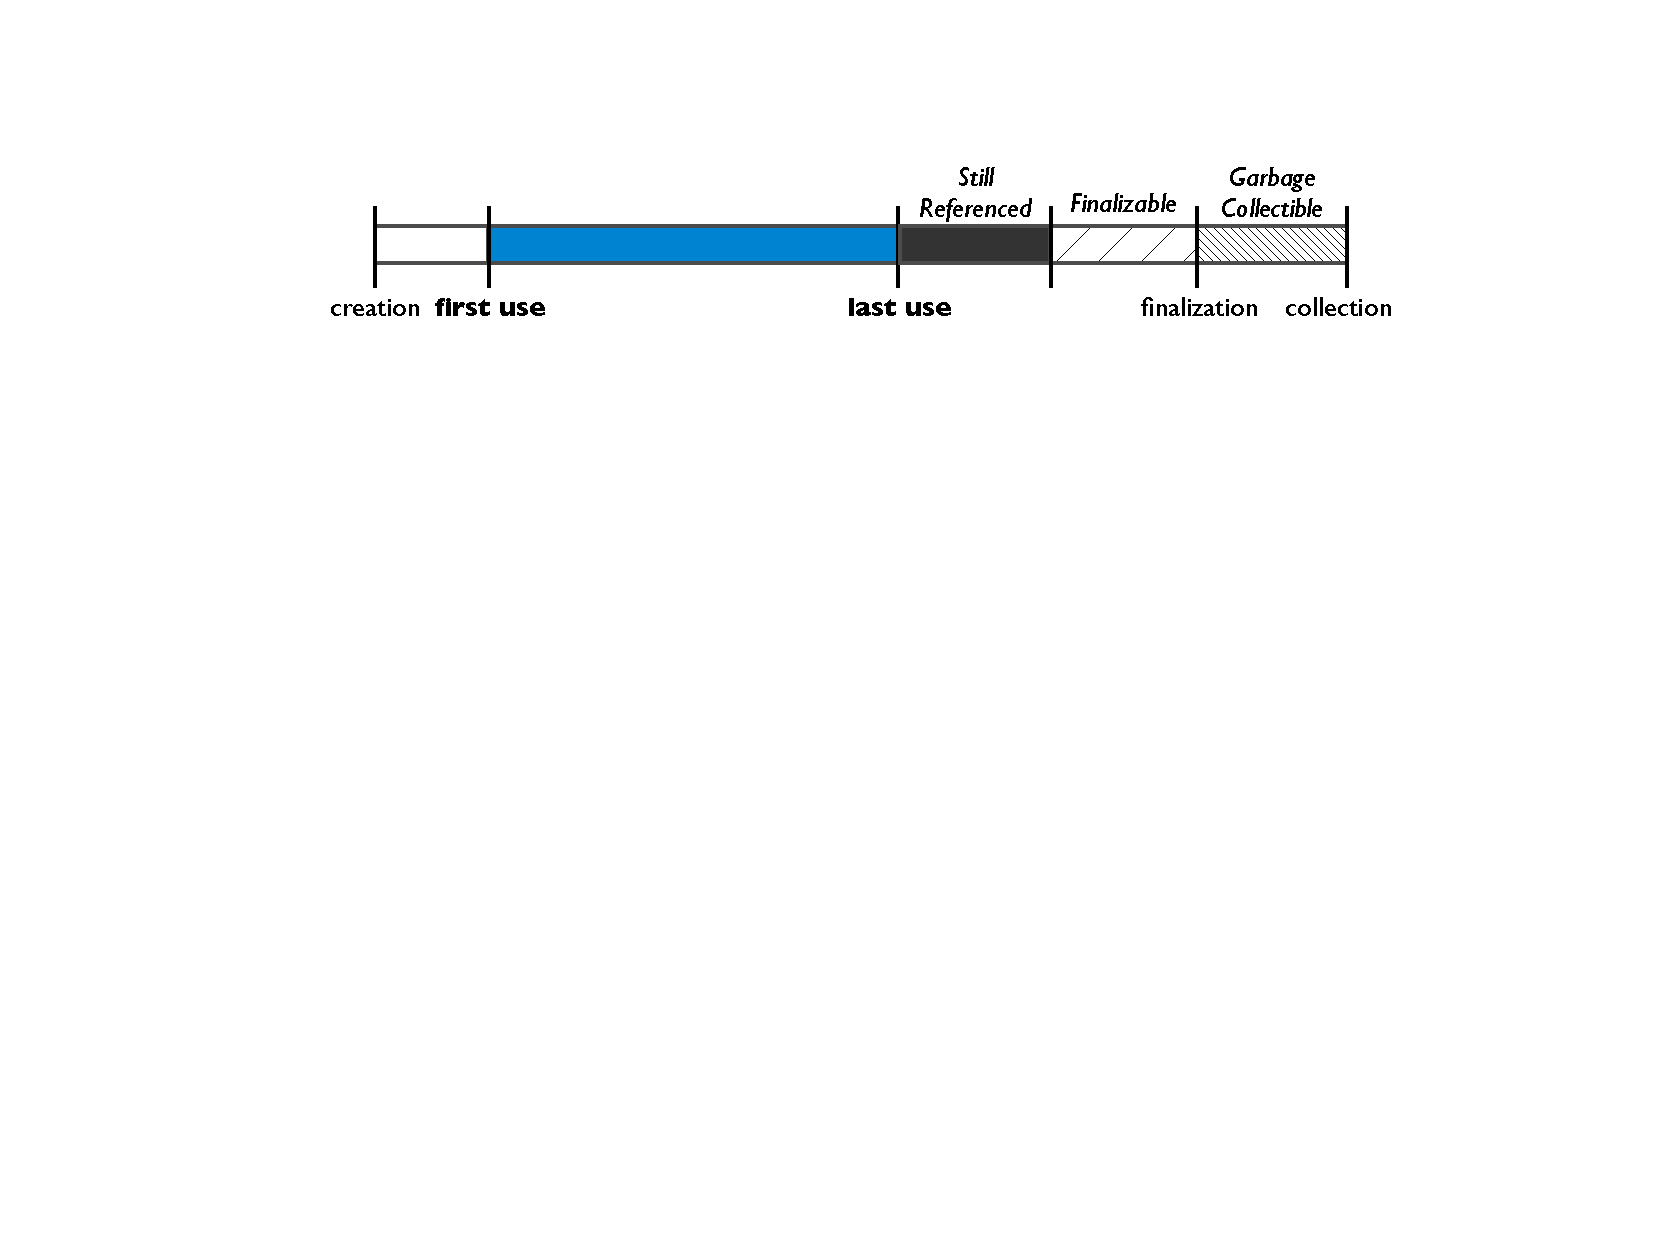
\includegraphics[width=0.95\textwidth]{part2/Figures/lifetime/object-lifecycle}
	%}
	\subfigure[A situation where there are long periods between uses of an
	object's data.]{
	\label{fig:typical-lifecycle2a}
		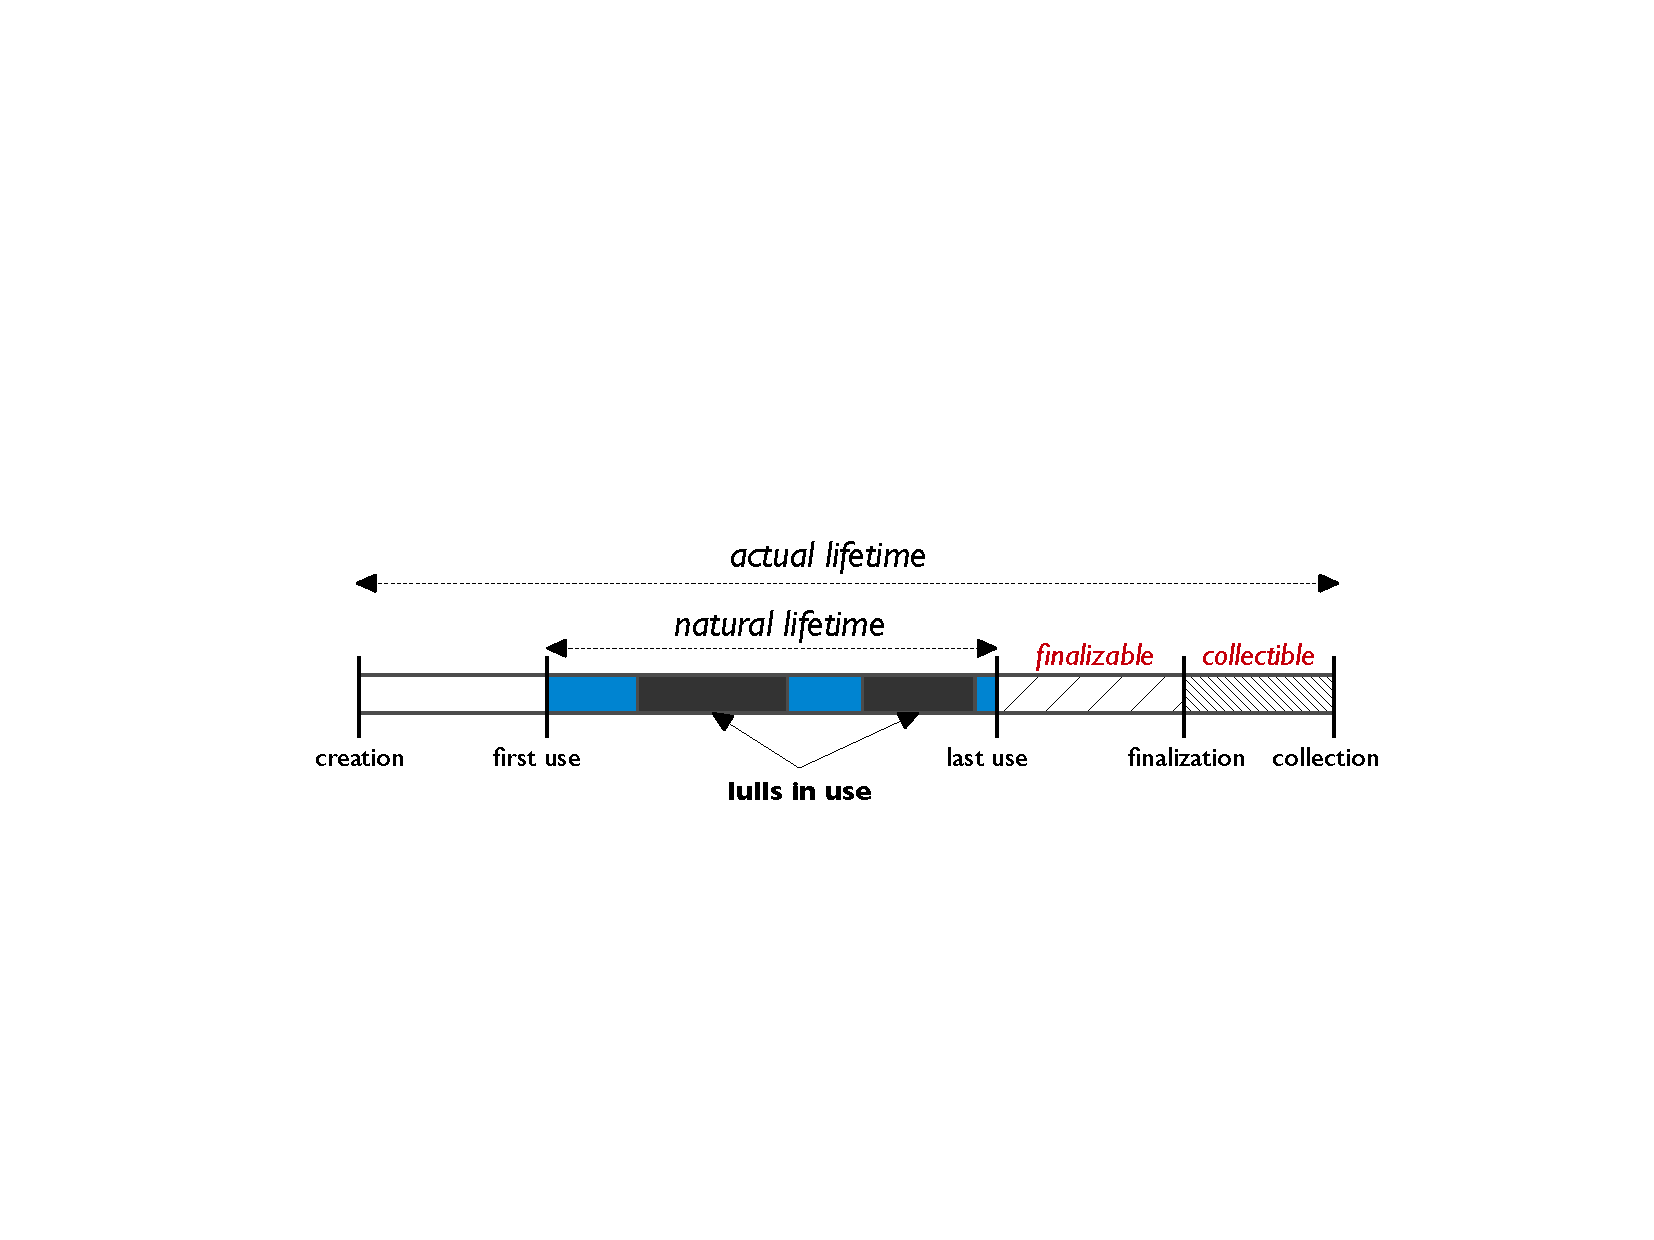
\includegraphics[width=0.95\textwidth]{part2/Figures/lifetime/object-lifecycle-lulls}
	}
	\subfigure[The lifecycle of the data  that is loaded from
	disk three times, and the objects that store it.]{
	\label{fig:typical-lifecycle2b}
		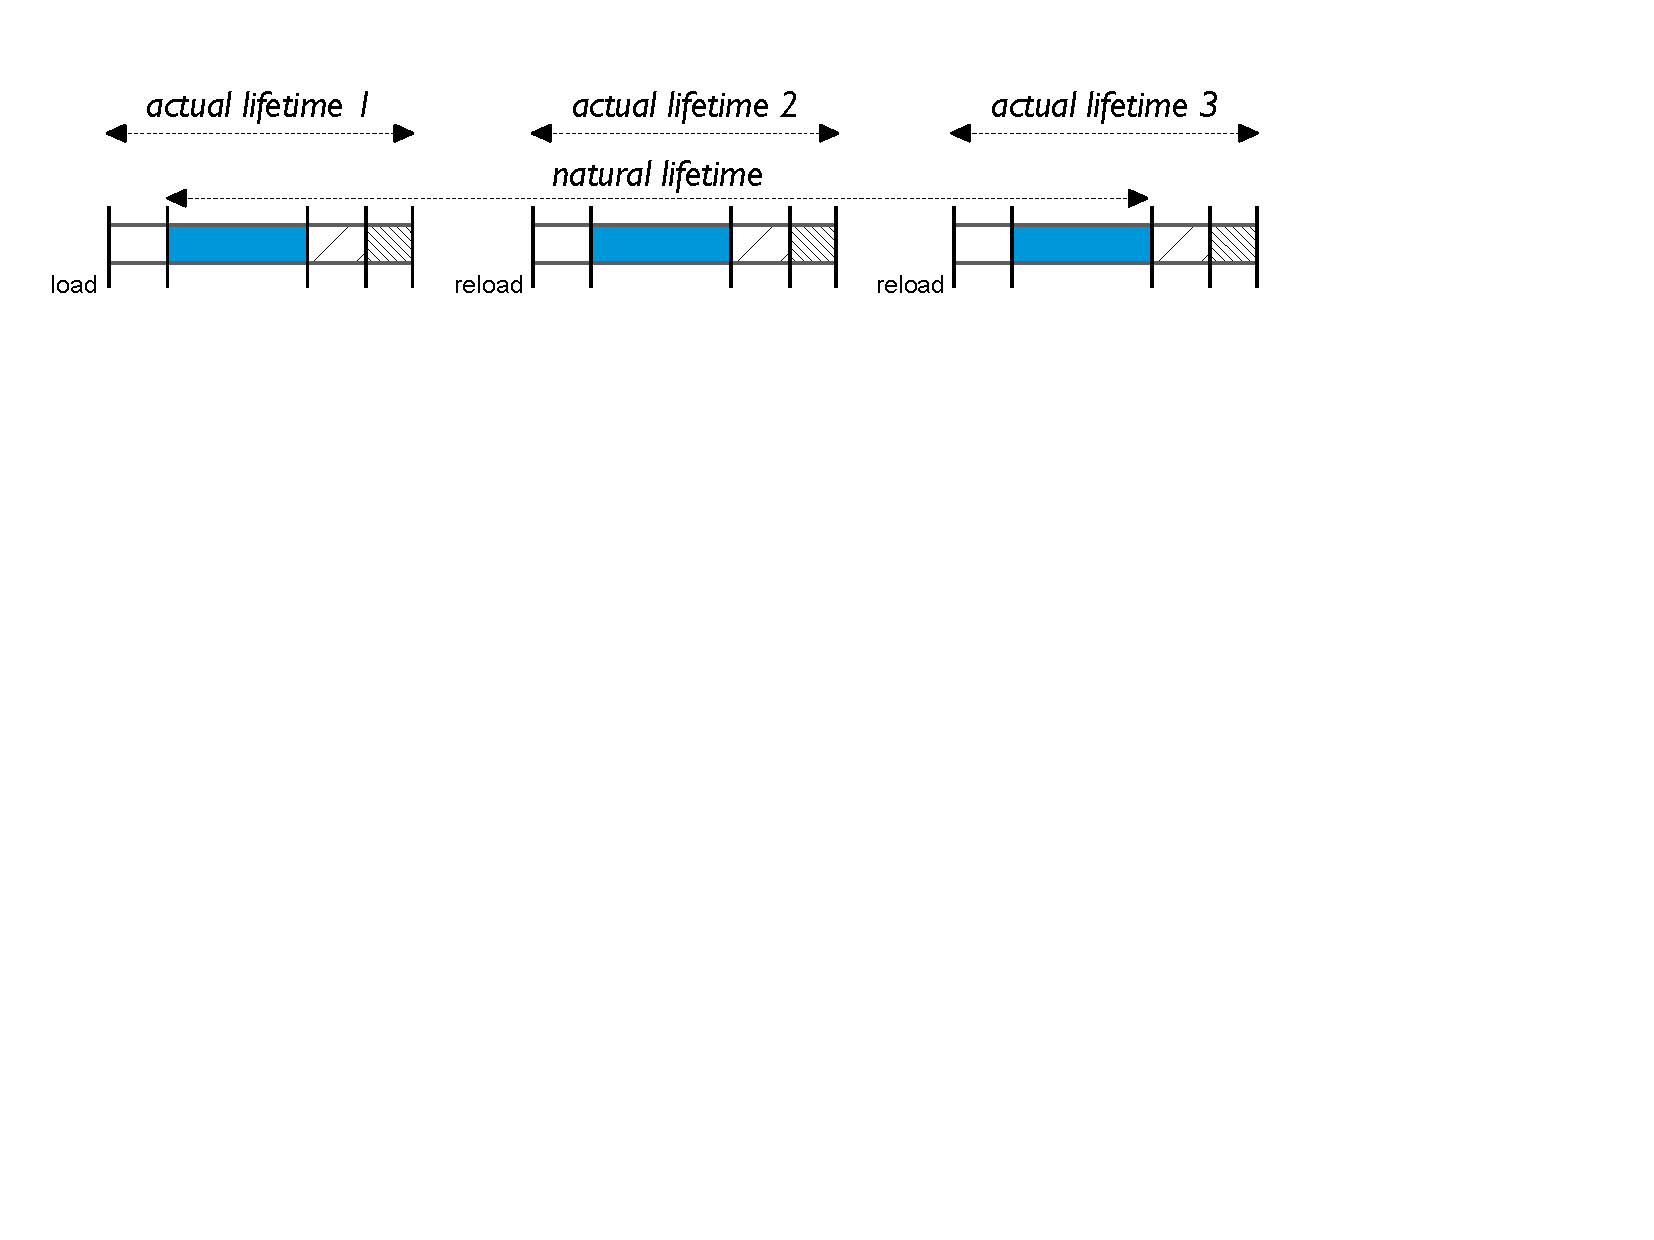
\includegraphics[width=0.9\textwidth]{part2/Figures/lifetime/object-lifecycle2}
	}
	\caption{Examples of Natural and Actual lifetimes.}
	\label{fig:typical-lifecycle2}
\end{figure}
\end{comment}


\paragraph{Shared Ownership}
\label{sec:shared-ownership}
\index{Shared Ownership}

When you invoke a library method, there is no way in Java to know what the called
method does with your object. It could very well squirrel away a reference to any
object reachable from arguments you pass to the invocation. Despite your best
efforts at keeping track of which references exist to an object, it can easily
become an uncontrolled mess once you pass these objects to third-party libraries.
In the above example, if you call the \code{parse} method of a
\class{SimpleDateFormat} object, the method contract says nothing about how it
treats the given string or \class{ParsePosition} passed as parameters. 
Consider the case where you need the string to become garbage collectable soon
after having parsed it, but the formatter maintains a reference in order to avoid
reparsing the same string in back to back calls. This calls
to mind the worst of the days of explicitly managing memory in a language like C.

In the case where there is more than one reference to the object, the story gets
more complicated. In contrast to C, where a \code{free} of \emph{any} pointer
suffices for deallocation, in Java \emph{all} references to an object must be
assigned to \code{null}. This is tricky in many cases, because it may not be easy
to know where all those references emanate from.
\autoref{fig:reachability-sharing} illustrates a situation where three references
must be clipped before an object, the darkly shaded one, becomes a candidate for
garbage collection. There are two other important things to note in this example.
First, just as in \autoref{fig:reachability-b}, after clipping the three
indicated references, an entire data structure, not just that darkly shaded
object, becomes a candidate for reclamation. This structure consists of the two
objects contained within the lightly shaded region. The second important thing to
note is that you needn't clip the backwards edge, or any edge contained entirely
within the data structure you no longer need.

\begin{figure}
\centering
\subfigure[Diamond sharing.]{
	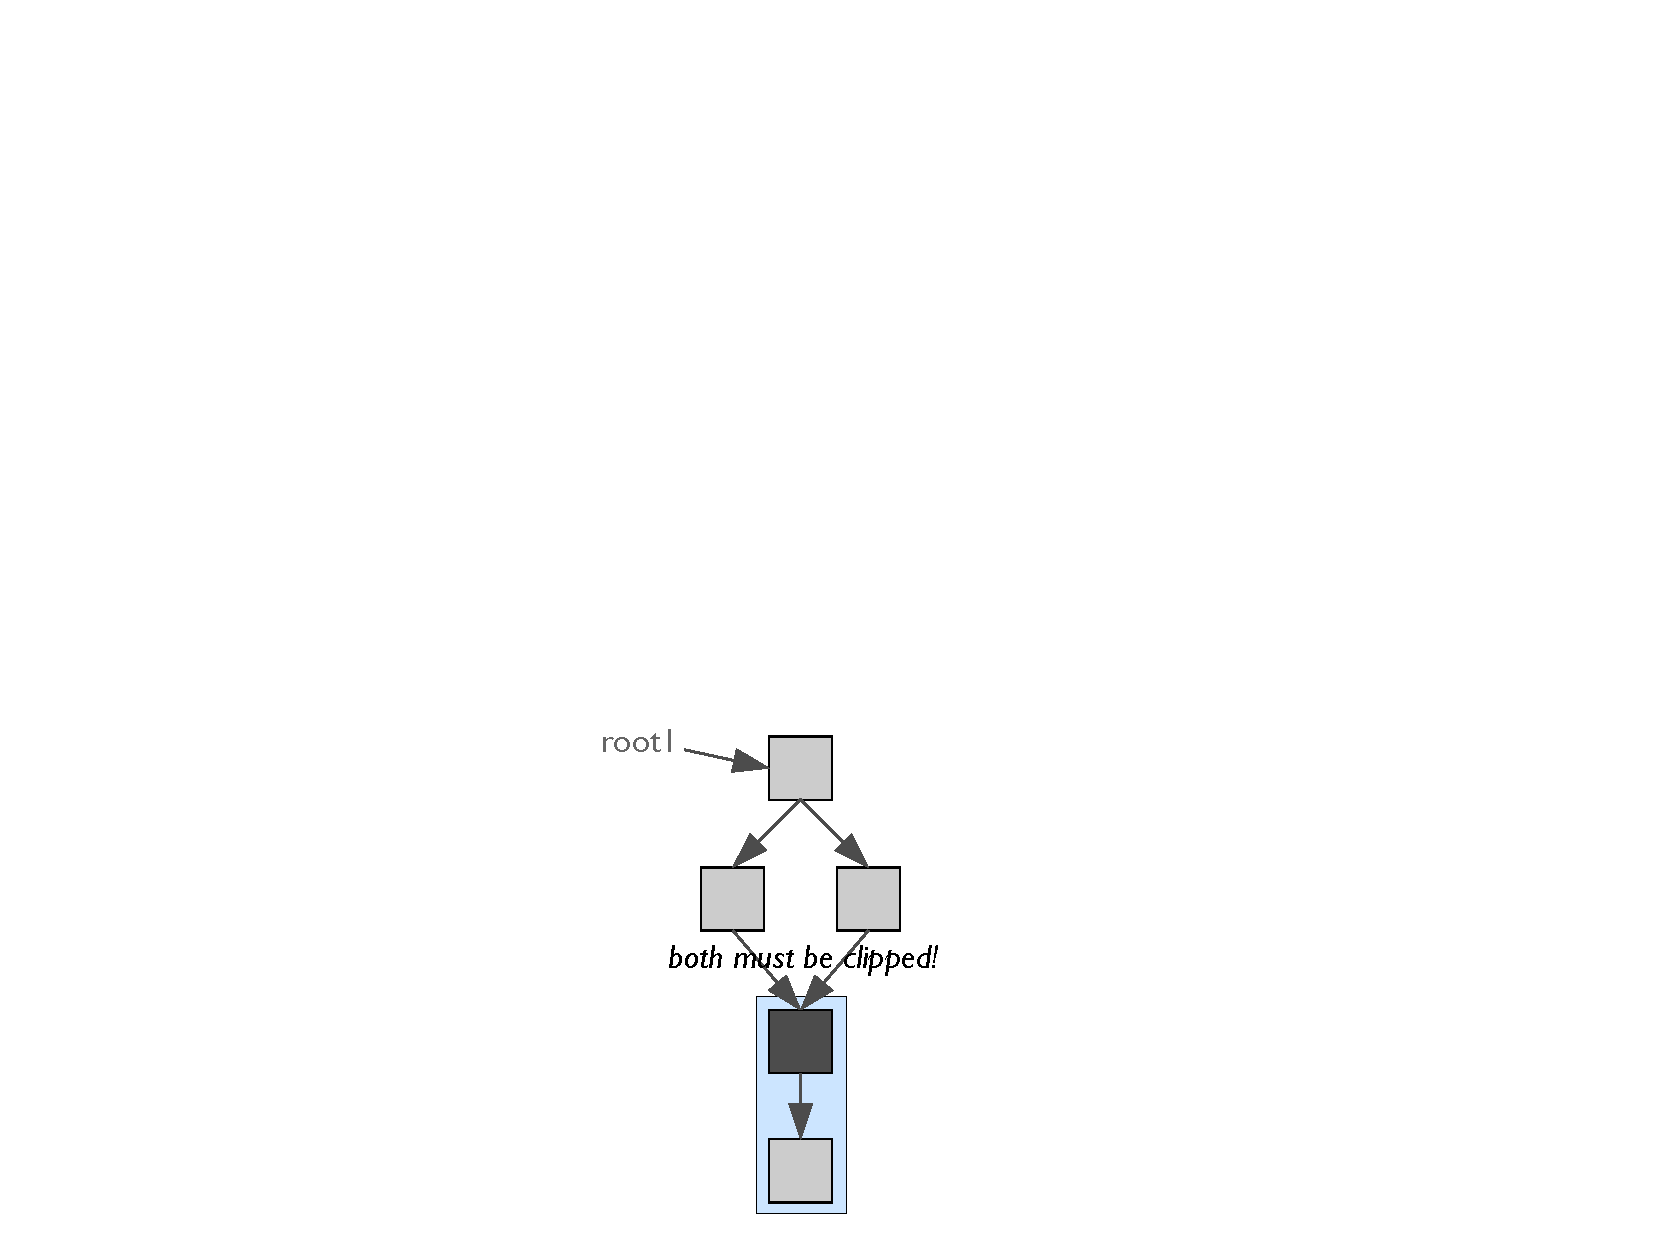
\includegraphics[height=0.25\textheight]{part2/Figures/lifetime/reachability4}
	}
\qquad
\subfigure[Root sharing.]{
	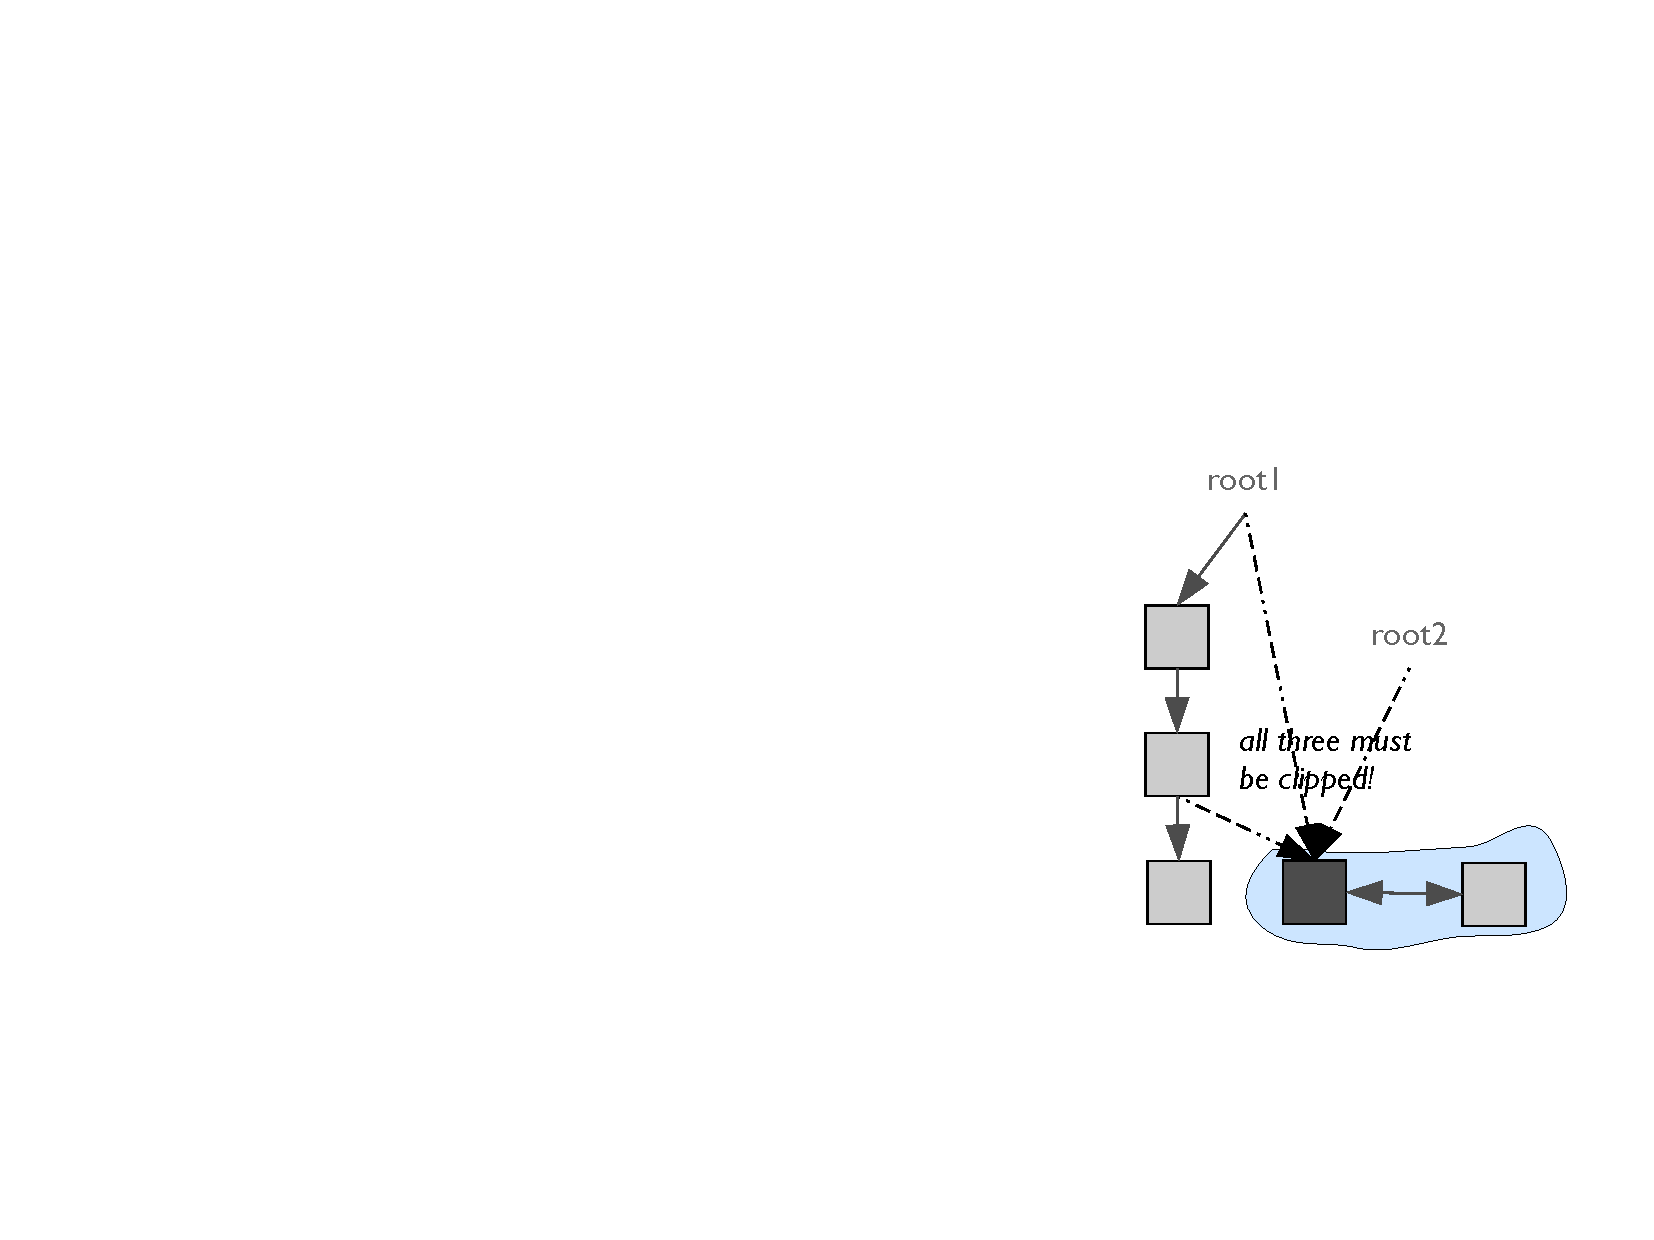
\includegraphics[height=0.22\textheight]{part2/Figures/lifetime/reachability3}
	}
	\caption{When an object is shared, such as the shaded ones shown
	here, care must be taken to clip all edges from emanating from outside of the
	region you wish to reclaim.}
	\label{fig:reachability-sharing}
\end{figure}

\section{Lifetime Management: Beyond Reachability}
Sometimes, you need an object to stay alive, or not, in a way that has nothing
to do with whether it is reachable from local variables or static fields. For
example, to implement the correlated lifetime policy described in
\autoref{sec:correlated-lifetime} using only the mechanisms presented so far is
difficult. 

Using reachability, the only way to guarnatee that one object
$B$ will become a candidate for garbage collection when another object $A$ does,
would be to have $A$ dominate $B$. Sometimes this can work, but more often,
this is not possible. Doing so requires modifying $A$, or something that $A$
domiantes, so that it points to $B$. But what if you don't own any of that code?
\autoref{fig:reachability-b} illustrates an example of this. There are three
objects contained within the shaded region; these three objects will all be garbage collectible if
the indicated dominating reference is set to \code{null}. In this way, the
lifetime of the lower two can be correlated with the lifetime of the object
directly pointed to by the dominating reference.

In addition to requiring the pollution of class definitions, it also can result
in wasted memory. If only some \class{A} instances have a correlated \class{B},
then you will be wasting a pointer slot for every instance of \class{A}. It turns
out that this is how the Java standard \class{HashMap} was implemented, in its
mechanism for maintainin a correlation between the various views (the key set,
value set, and entry set), and the map itself:
\begin{shortlisting}
class HashMap {
   Set keySet, valueSet, entrySet;
}
\end{shortlisting}
This choice had a big implication on the memory bloat factor of small maps. As
we have learned in previous chapters, every instance of a standard Java hash map
must pay the expense for potential use of features. These features aren't
always employed, and certain rarely together, for a single map instance.

The Java language provides mechanisms that allow you more flexibility in
implementing lifetime management policies. These advanced features are exposed
via soft, weak, and phantom references, finalization, and \tls.
In contrast, the term used for 
the
normal way of referencing objects, that is what you get when you use fields of
objects or local variables, is a \emph{strong}
reference\index{Reference, Strong}.

\paragraph{Soft and Weak References}
\index{Reference, Weak}
\index{Reference, Soft}
% Programmers
%very often confuse these mechanisms, and there is quite a bit of disinformation
%on the Internet; there is especially confusion over the use of soft and weak
%references.

Soft and weak references are two alternate ways for one object to reference
another. If one object strongly references another, then the normal garbage
collection rules apply. If one object \emph{softly references} another, then
the garbage collector is free to clip that reference whenever it wants. Once the
garbage collector decides to make that reference go away, then the normal rules
of reachability apply; if it is not reachable from static fields or local
variables, then it is collectible.
A \emph{weak} reference acts like a reverse strong reference. In the case of a
normal strong reference from object $A$ to object $B$ (assuming no other
references to $B$), once $A$ is collected, $B$ becomes collectible. If $A$
weakly references $B$, then once $B$ becomes collectible, $A$ becomes
collectible --- just the reverse of a normal strong reference! In this way, weak
references can form the basis of the implementation of correlated lifetime
patterns.

``Soft'' and ``weak'' are strange terms, but the rules are pretty much as simple
as that. Programmers are often confused by these two, and the web searches will
reveal some degree of misinformation. It is common for web sites misdefine
these two mechanisms, e.g. by swapping their roles. In short:

\callout{softweak}{Soft and Weak References}{ If one object \emph{softly
references} another, then the garbage collector is free to clip that reference
whenever it wants. A \emph{weak} reference acts like a reverse strong reference.
 }
 
The Java language specification places no firm criteria upon \jre
implementations as to when they should clip soft references. In practice, soft
references won't be clipped at the random whim of the \jre. All \jres these days
will attempt to clip soft references in a roughly LRU (least-recently used)
fashion: soft references that haven't been traversed in a while will be clipped
before those that are frequently used. In this way, soft references can form the
basis for cache implementations.

You should not use these references lightly. \autoref{tab:reference-costs}
summarizes the costs of the ways of one object referencing another. A strong
reference costs one pointer, which is 4 bytes (32 bits) on a 32-bit \jre. In
comparison, a weak reference is \emph{eight times} more costly, at 32 bytes per
reference, and a soft reference is nine times more costly. The reason for these
expenses is that you must create an extra \class{Reference} object for
every soft or weak reference you use. To softly reference a date formatter,
you would write:
\begin{shortlisting}
void foo(DateFormat dateFormatter) {
   SoftReference<DateFormat> ref = new SoftReference<DateFormat>(dateFormatter);
   ...
}
\end{shortlisting}

\begin{table}
\centering
	\begin{tabular}{ll}
		\toprule
		reference type & memory cost \\
        \cmidrule(r){1-1} \cmidrule(l){2-2}		
		strong         & 4 bytes (one pointer) \\
		finalization   & 28 bytes \\
        phantom        & 32 bytes \\ 
		weak           & 32 bytes \\
		soft           & 36 bytes \\
		\bottomrule
	\end{tabular}
	\caption{The cost, per reference, of the various ways of one object
	referencing another.}
	\label{tab:reference-costs}
\end{table}

% 32 is: the 4 pointer fields of java.lang.ref.Reference = 16
%   plus an object header = 12
%   plus the pointer to the Reference object itself = 4

\paragraph{Reference Queues}
Normally, when you create a soft reference, and the \jre decides to clip it,
then the associated \class{Reference} object becomes immediately garbage
collectible. You get no warning that the \jre has clipped this reference.
Sometimes, this is good, because it lets you very easily take advantage of the
soft and weak referencing mechanisms. More often, however, your code will need
some warning that a reference has been clipped. For example, if you are using
soft references to implement a cache (this is discussed in more detail in
subsequent chapters), then you will probably need to perform some cleanup work
when the reference is clipped.

Java provides reference queues for exactly this purpose. When you construct a
soft or weak reference, and associate it with a reference queue, then something
different happens when the reference is clipped. Instead of becoming
collectible, when clipped, it is placed on the associated reference queue. It is
your job to periodically \emph{poll} the reference queue in order to enquire as
to whether any references have been clipped. If this somes tedious and error
prone, it is! Subsequent chapters show how to get it right.

Another point of caution: reference queues add an extra pointer to the already
high memory expense of using soft or weak references. For example, a weak
reference with an associated reference queue would cost 36 bytes per reference.

\paragraph{Handling External Resources: Finalization and Phantom References}
\index{Finalization of objects}

Weak references can help you to correlate the life of one object with that of
another. Sometimes, it is necessary instead to correlate an \emph{action} with
the reclamation of an object. This is helpful if there are non-Java resources
associated with a Java object that need to be cleaned up along with that object.
The JVM knows nothing about those resources, since they aren't Java objects;
they may not even be memory, per se, or may be memory on an entirely different
machine. For example, a Java \class{DatabaseConnection} object has implicit
linkage to a whole slew of resources, scattered across several machines. There
are operating resources on the local machine that are involved. The remote
database machine has these, too, and the database process also has some
internal state about that connection. All of this state needs to be cleaned up
when the Java facade for it is reclaimed.

Java assumes a closed world about resources. As long as the resources fall
within its boundaries, then the automated mechanisms, such as garbage
collection, work well, without much intervention on your part. For these
more complex cases, such as a database connection, the nice fully automated
world start to fall apart a bit.
One recourse is to fall back to the C style of resource management, for these
cases of external resources. You can design the API specifications so as to
require users of the API to adopt a convention that requires explicit closing,
or freeing of resources. 

Java provides \emph{finalization} as a way around this problem, though it comes
with many gotchas. Finalization is very much like the system of weak references,
in that it is a way to correlate an action with the death of an object. If you
write a class with a \code{finalize} method, then, when that object is
reclaimed, the finalize method will be called. Behind the scenes, the \jre
allocates an extra object (of type \class{java.lang.ref.FinalReference}) and
stores these in a reference queue (called the finalization queue). Phantom
references are a minor variation of finalization that lets you manage the queues
more flexibly: you can use separate queues for different groups of objects, and
manage how often to poll the queues, rather than having a single queue and
relying on the \jre to poll the queue when it feels like it.\index{References,
Phantom}

Now for the gotchas. First, you can't assume that the finalize method will be
called immediately after the correlated objects death. The Java language
specification does not dictate a timeliness criterion for invoking your
\code{finalize} method. This can lead to dragging of the resources, exactly like
the problem of memory drag described earlier. Second, using finalization
increases memory bloat. For every instance of a class with a \class{finalize}
method, the \jre, behind the scenes, allocates an extra object (of type
\class{java.lang.ref.FinalReference}). This object consumes 28 bytes; the
pointer from the finalization queue adds an extra pointer cost.
\index{Overwhelming the Finalizer Thread}
Third, it is possible to overwhelm the finalization thread. This can happen if
your program creates instances of objects with \code{finalize} methods at a high
rate.
\begin{comment}
 Such is the
case in the following loop:
\begin{shortlisting}
import java.awt.Font;
for (int i = 0; i < N; i++) {
   Font font = new Font("SansSerif", Font.BOLD, 12);
   ... // some small amount of work
   // font does not escape the loop
}
\end{shortlisting}
Since each loop iteration's instance of \code{font} is not used beyond the
execution of that iteration, it seems like one could run this program on a
small heap, for any value of \code{N}. The heap need only fit what it
takes to allocate the handful of objects that represent an instance of
\code{java.awt.Font}. Try it out, for various values of \code{N} and of
\code{-Xmx}! On Sun and IBM Java 6 \jres, you will find that, as \code{N}
increases, you will need to increase the maximum heap size allotted to the \jre.
If you don't, this code will fail with a \class{java.lang.OutOfMemoryError}.

The problem, in this case, is that \class{Font} class has a \code{finalize}
method. Therefore, as the loop iterates, instances of \class{Font} begin to pile
up the finalization queue. Periodically, the background finalizer thread wakes
up and cleans up the backlog. But, if this loop nest creates many \class{Font}s
quickly, or there are a large number of threads doing so concurrently, 
the finalizer background thread becomes overwhelmed. Try sticking in this code:
\code{if (i \% 100000 == 0) System.runFinalization()}. Here, you are explicitly
putting your application's thread to sleep in order to let the finalizer thread
catch up. In this case, this change fixes the problem.
\end{comment}

\paragraph{\TLS}
\tlsindex % \index{\TLS} doesn't seem to work
When you reference an object from a static field of a class, the object will
stay around pretty much for the life of the program. While this lets you
implement a permanently resident lifetime pattern, it is not thread safe. In
order to protect write access to static fields, you will need to guard these
operations with locks. This is possible, but tedious and often results in poor
performance due to contention of threads trying to acquire those locks: they
need to sleep before they can enter the contended critical section.

Java provides an alternative way to implement a permanently resident pattern
called \emph{\tls\/}. \tls provides a way to clone data so that each thread has
its own copy. It is impossible for one thread to access another thread's local
storage. When you store objects in a thread's local storage, the objects will
live for as long as the thread does, unless you \code{null} them out or
otherwise otherwrite the entries first.

To use \tls, you need to create a \emph{thread-local variable}. A thread-local
variable represents a piece of data that you want to clone across threads. For
example, if you'd like each thread to have it's own date formatter, because your
date formatter isn't thread safe, then you would create a thread-local variable
for it:
\begin{shortlisting}
class C {
   static ThreadLocal<DateFormat> dateFormatter = new ThreadLocal<DateFormat> {
      protected DateFormat initialValue() {
         // called the first time a thread tries
         // to access this thread-local variable
         return new ...;
      }
   };
   
   String format(Date d) {
      return dateFormatter.get().format(d);
   }
}
\end{shortlisting}
The main thing you have to be cautious of is memory drag. If you store a large
structure in the local storage of a thread that lasts for the duration of the
program, but only use the structure early in your program's execution, then that
structure will be needlessly consuming space. Your options are either to design
things so that the thread terminates, rather than staying alive forever; or you
can explicitly overwrite the entry, by calling {\tt dateFormatter.put(null)},
but this must be done by the thread itself, since there is no way for one thread
to access another thread's local storage; or, finally, you can have the
thread-local variable store a soft reference to the data:
\begin{shortlisting}
ThreadLocal<SoftReference<DateFormat>> dateFormatter;
\end{shortlisting}
Now, each thread's copy of the date formatter will be cleaned up by the garbage
collector if it ever needs the space, and the formatter hasn't been used in a
while. You need to take care to handle the case when the \jre does get around to
clipping the soft reference, and you come back to format new dates. Still, this
hybrid approach, of combining soft references and \tls, can be quite powerful.

\section{Summary}


\begin{itemize}
  \item Every Java process has multiple memory regions, each with separate size
  limits and separate configuration options for adjusting these limits.
  \item Local variables in Java programs can only store primitive data and
  pointers to heap-allocated objects.
  \item Memory leaks can easily occur in a Java application, despite it having a
  garbage collector.
\end{itemize}